\documentclass[12pt,a4paper]{article}
\usepackage[T1]{fontenc}
\usepackage[utf8]{inputenc}
\usepackage[polish]{babel}
\usepackage{lmodern}
\usepackage{geometry}
\usepackage{graphicx}
\usepackage{booktabs}
\usepackage{float}
\usepackage{siunitx}
\usepackage{hyperref}
\usepackage{subcaption}
\usepackage{array}
\usepackage{longtable}
\usepackage{caption}
\geometry{margin=2.2cm}
\sisetup{
  output-decimal-marker={,},
  group-separator={\,},
  group-minimum-digits=4
}
\hypersetup{
  colorlinks=true,
  linkcolor=black,
  urlcolor=blue
}
\title{Sprawozdanie z laboratorium 0.}
\author{Jakub Kogut}
\date{\today}

\begin{document}
\maketitle

\section{Cel ćwiczenia}
Celem ćwiczenia było porównanie bardzo prostego podejścia losowego z heurystyką opartą
na minimalnym drzewie rozpinającym dla euklidesowego problemu komiwojażera (TSP).
Zgodnie z treścią zadania należało dla instancji \texttt{wi29}, \texttt{dj38}, \texttt{qa194},
\texttt{uy734} i \texttt{zi929}:
(1) wylosować \num{1000} permutacji wierzchołków i policzyć trzy statystyki,
(2) przygotować skrypt do graficznej prezentacji rozwiązań,
a dodatkowo
(3) policzyć MST i jego wagę oraz
(4) zbudować cykl TSP z kolejności pierwszego odwiedzenia wierzchołków w przeszukiwaniu DFS po MST.

\section{Opis metody}
Dane pochodzą z kolekcji Waterloo World TSP, gdzie wagi są liczone jako odległości euklidesowe
zaokrąglane do najbliższej liczby całkowitej zgodnie z normą \texttt{EUC\_2D}.
Dla każdej instancji wykonano następujące kroki:
\begin{enumerate}
    \item wylosowano \num{1000} permutacji wierzchołków,
    \item policzono średnią z minimów dla \num{100} kolejnych grup po \num{10} losowań,
    \item policzono średnią z minimów dla \num{20} kolejnych grup po \num{50} losowań,
    \item wyznaczono minimum globalne spośród wszystkich \num{1000} losowań,
    \item zbudowano minimalne drzewo rozpinające algorytmem Prima,
    \item wykonano przeszukiwanie DFS po drzewie i z kolejności pierwszych odwiedzin utworzono cykl Hamiltona
\end{enumerate}

\section{Odpowiedzi na pytania z treści zadania}
\subsection*{Dlaczego nie \texorpdfstring{$n!$}{n!}?}
Jeżeli reprezentujemy cykl przez permutację, to ten sam cykl można zapisać na \emph{n}
sposobów przez cykliczne przesunięcie punktu startowego. Po ustaleniu pierwszego wierzchołka
pozostaje więc \((n-1)!\) reprezentacji. 

\subsection*{Czy w optymalnej pętli euklidesowej krawędzie mogą się krzyżować?}
Nie. Jeżeli dwie krawędzie cyklu się przecinają, to można zastosować operację typu 2-opt,
czyli zastąpić je dwiema nieprzecinającymi się krawędziami. W przestrzeni euklidesowej,
na mocy nierówności trójkąta, taka zamiana skraca trasę. Zatem cykl optymalny nie powinien
zawierać przecięć. To od razu wskazuje prostą możliwość poprawy losowych tras:
lokalne usuwanie przecięć powinno istotnie zmniejszać ich długość.

\subsection*{Dlaczego waga MST jest mniejsza od kosztu optymalnego cyklu TSP?}
Po usunięciu dowolnej krawędzi z cyklu Hamiltona otrzymujemy drzewo rozpinające.
Jego waga jest mniejsza od wagi tego cyklu o wagę usuniętej krawędzi, a więc w szczególności
nie przekracza kosztu optimum TSP. MST jest najtańszym spośród wszystkich drzew rozpinających,
stąd zachodzi:
\[
w(\mathrm{MST}) \leq w(T) \leq w(\mathrm{OPT}).
\]

\subsection*{Dlaczego cykl zbudowany z MST ma koszt nie większy niż dwukrotność kosztu drzewa?}
Gdy każdą krawędź drzewa przejdziemy dwa razy, otrzymamy spacer o koszcie \(2\,w(\mathrm{MST})\).
W metrycznym TSP, a więc także w wariancie euklidesowym, ``skrótowanie'' powtórzonych wierzchołków
nie zwiększa długości trasy. Z tego wynika klasyczne ograniczenie:
\[
w(\mathrm{DFS\ tour}) \leq 2\,w(\mathrm{MST}).
\]
Wyniki eksperymentu potwierdzają to dla każdej badanej instancji.

\section{Wyniki liczbowe}
W Tabeli~\ref{tab:random} zestawiono trzy wymagane statystyki dla losowych permutacji.
W Tabeli~\ref{tab:mst} pokazano wagę MST, koszt cyklu MST+DFS oraz -- dla porównania --
znane optimum z serwisu Waterloo World TSP.

\begin{table}[H]
\centering
\caption{Wyniki dla części losowej}
\label{tab:random}
\small
\begin{tabular}{@{}lrrrr@{}}
\toprule
Instancja & \(n\) & Śr. min 100$\times$10 & Śr. min 20$\times$50 & Minimum globalne \\ \midrule
Western Sahara (wi29) & 29 & \num{94815.56} & \num{88026.40} & \num{77380} \\
Dżibuti (dj38) & 38 & \num{24971.12} & \num{23339.50} & \num{21132} \\
Katar (qa194) & 194 & \num{88206.91} & \num{85875.60} & \num{82592} \\
Urugwaj (uy734) & 734 & \num{1596821.13} & \num{1578061.65} & \num{1560682} \\
Zimbabwe (zi929) & 929 & \num{2304806.75} & \num{2276382.80} & \num{2227257} \\
\bottomrule
\end{tabular}
\end{table}

\begin{table}[H]
\centering
\caption{Porównanie MST i cyklu MST+DFS z optimum}
\label{tab:mst}
\small
\begin{tabular}{@{}lrrrrrr@{}}
\toprule
Instancja & MST & MST+DFS & Optimum & Luka MST+DFS & MST/OPT & \(\frac{\mathrm{DFS}}{2\mathrm{MST}}\) \\ \midrule
Western Sahara (wi29) & \num{21753} & \num{34246} & \num{27603} & \num{24.07}\% & \num{78.81}\% & \num{0.787} \\
Dżibuti (dj38) & \num{5828} & \num{8737} & \num{6656} & \num{31.27}\% & \num{87.56}\% & \num{0.750} \\
Katar (qa194) & \num{8026} & \num{12446} & \num{9352} & \num{33.08}\% & \num{85.82}\% & \num{0.775} \\
Urugwaj (uy734) & \num{69873} & \num{106710} & \num{79114} & \num{34.88}\% & \num{88.32}\% & \num{0.764} \\
Zimbabwe (zi929) & \num{82863} & \num{131824} & \num{95345} & \num{38.26}\% & \num{86.91}\% & \num{0.795} \\
\bottomrule
\end{tabular}
\end{table}


W praktyce widać dwie bardzo wyraźne tendencje:
\begin{enumerate}
    \item Zwiększenie rozmiaru grupy z \num{10} do \num{50} zawsze poprawia wartość średniego minimum, bo
    w każdej grupie wybieramy najlepszy wynik z większej liczby prób.
    \item Losowe cykle bardzo szybko stają się bezużyteczne wraz ze wzrostem rozmiaru instancji:
    dla \texttt{uy734} i \texttt{zi929} minimum globalne z \num{1000} losowań jest odpowiednio około \num{19.73}
    i \num{23.36} razy większe od optimum. Dla porównania, heurystyka MST+DFS daje trasy tylko o około
    \num{24}--\num{38}\,\% gorsze od optimum.
\end{enumerate}

\section{Wykresy porównawcze dla części losowej}
Na Rysunkach~\ref{fig:avg10}--\ref{fig:overall} pokazano trzy osobne wykresy porównujące
instancje między sobą. Skala osi pionowej rośnie bardzo szybko dla dużych danych, co samo w sobie
dobrze ilustruje, jak słabe jest czysto losowe generowanie cykli.

\begin{figure}[H]
    \centering
    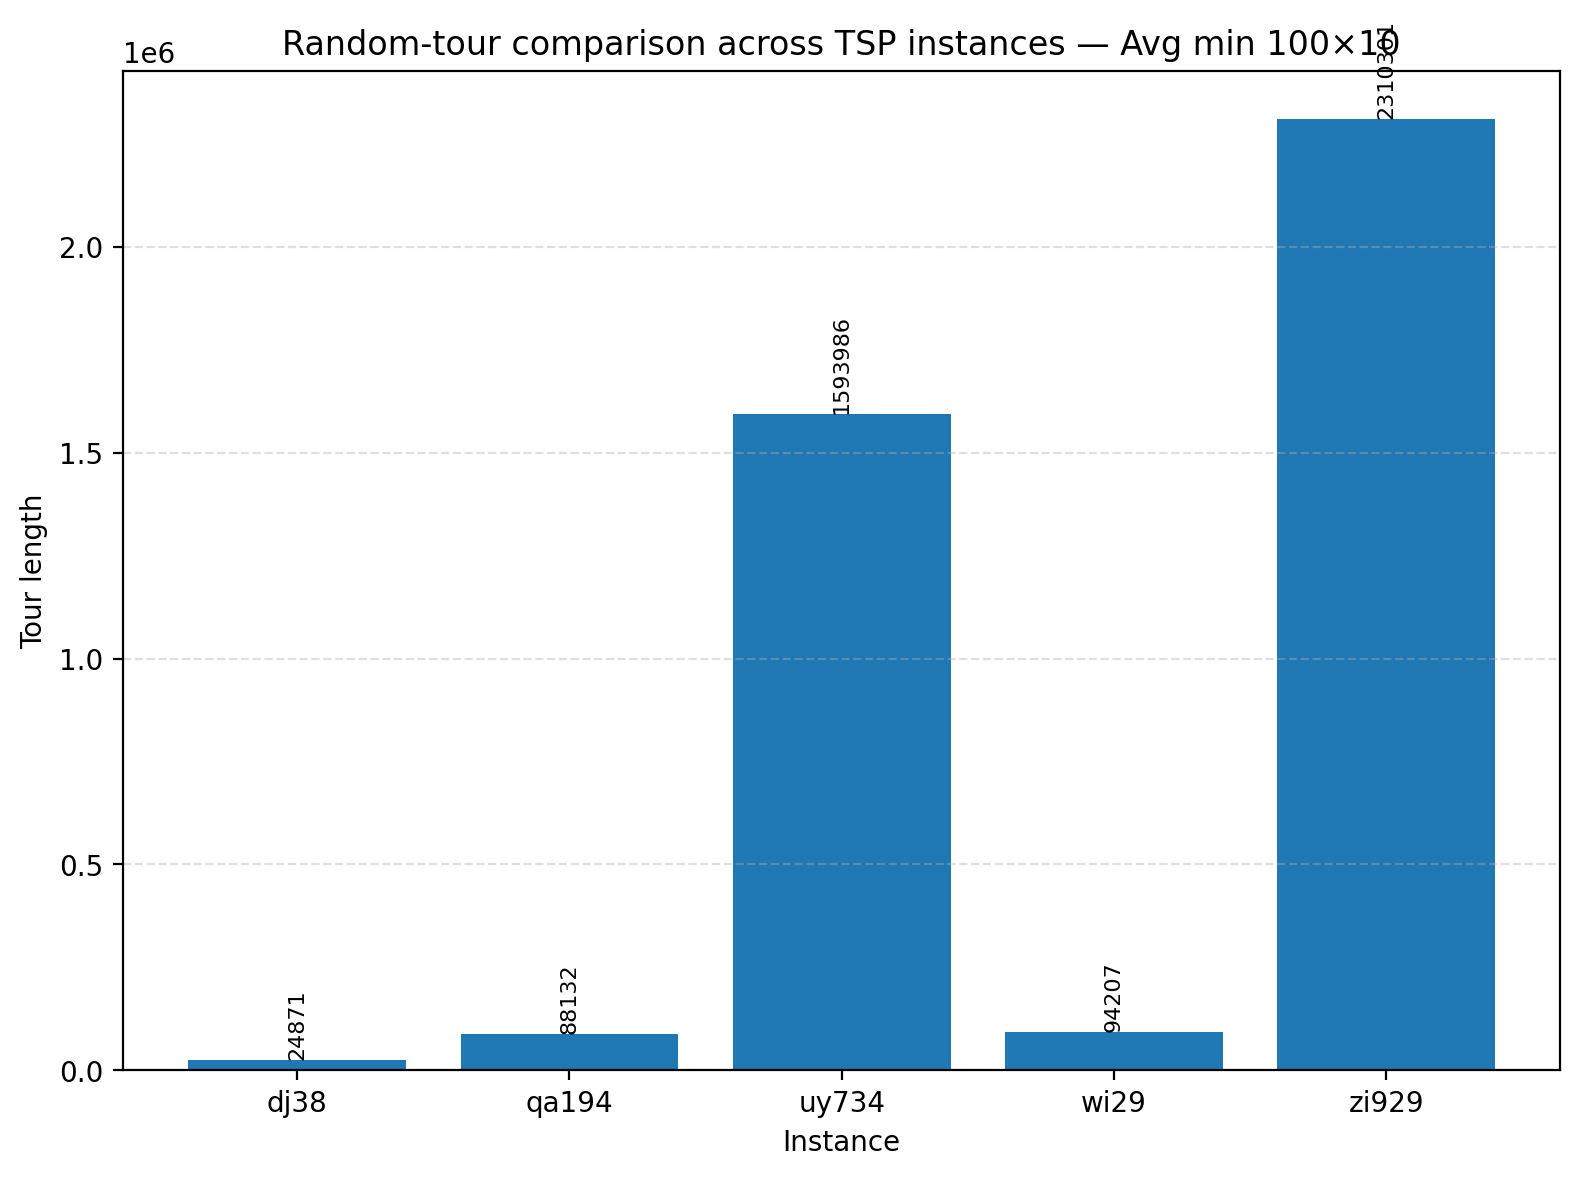
\includegraphics[width=0.86\textwidth]{plots_stats/avg_min_100x10.png}
    \caption{Porównanie wartości ``średnia z minimów dla 100 grup po 10 losowań''.}
    \label{fig:avg10}
\end{figure}

\begin{figure}[H]
    \centering
    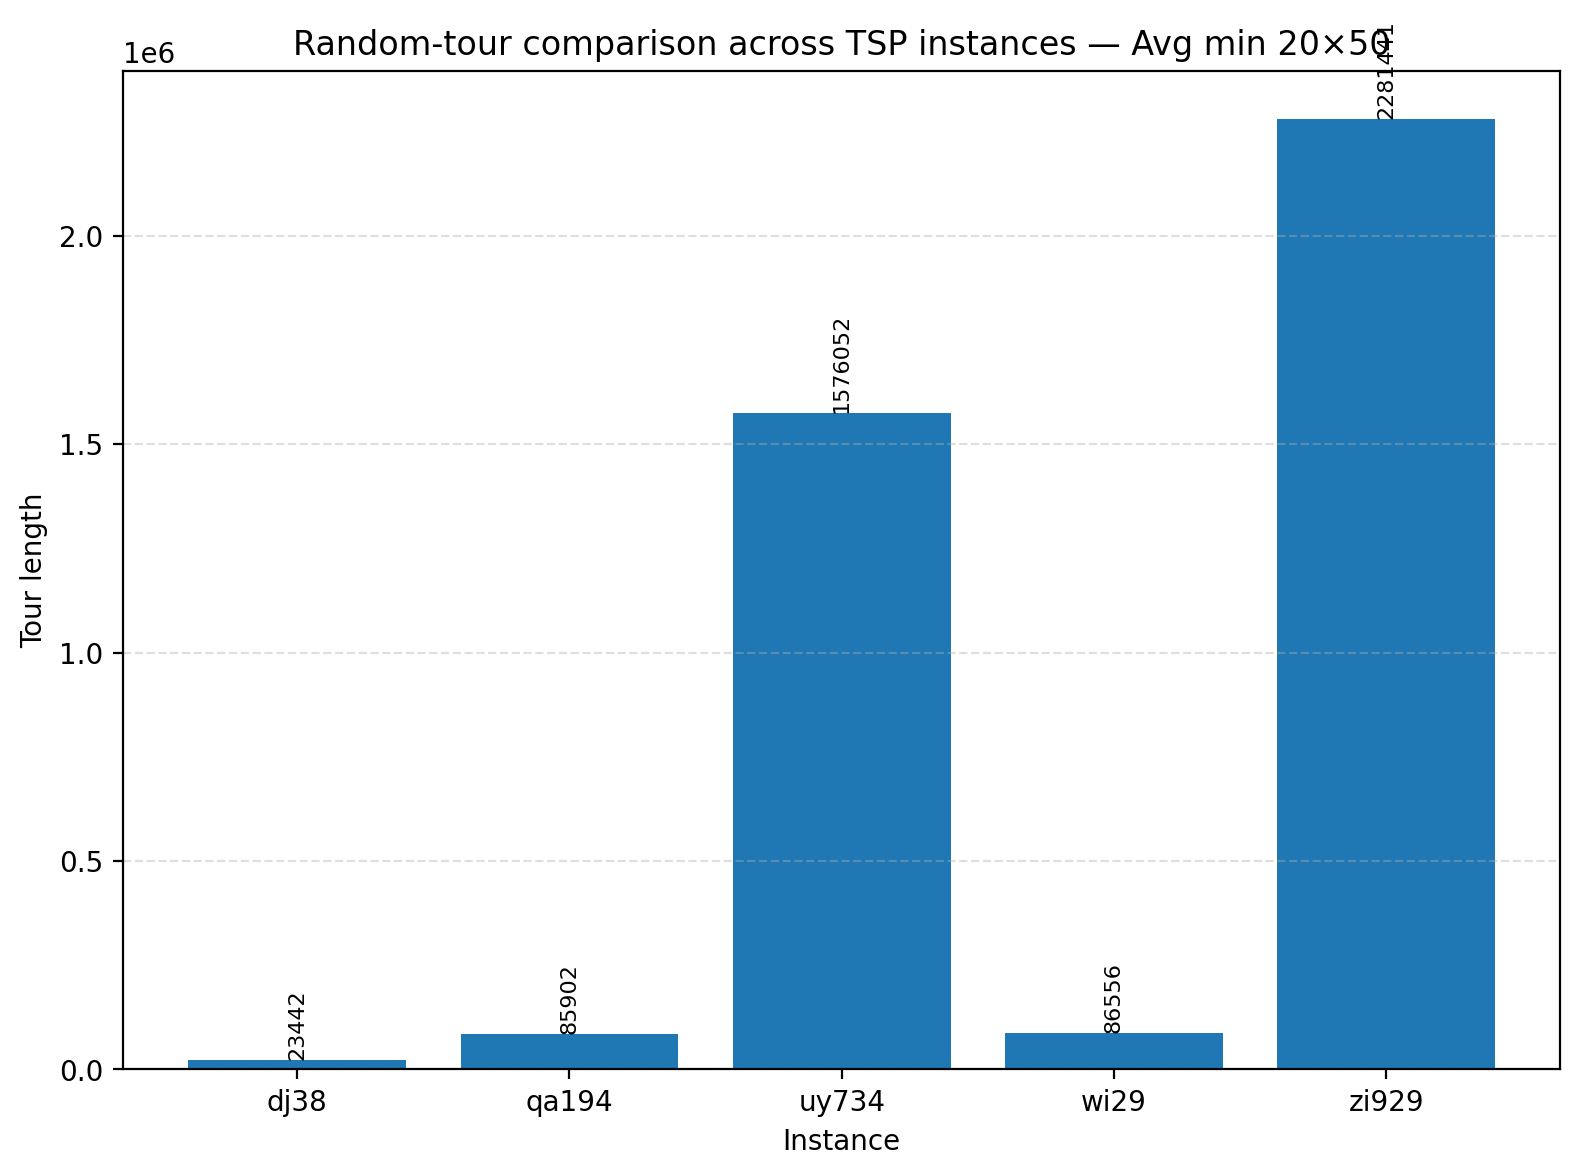
\includegraphics[width=0.86\textwidth]{plots_stats/avg_min_20x50.png}
    \caption{Porównanie wartości ``średnia z minimów dla 20 grup po 50 losowań''.}
    \label{fig:avg50}
\end{figure}

\begin{figure}[H]
    \centering
    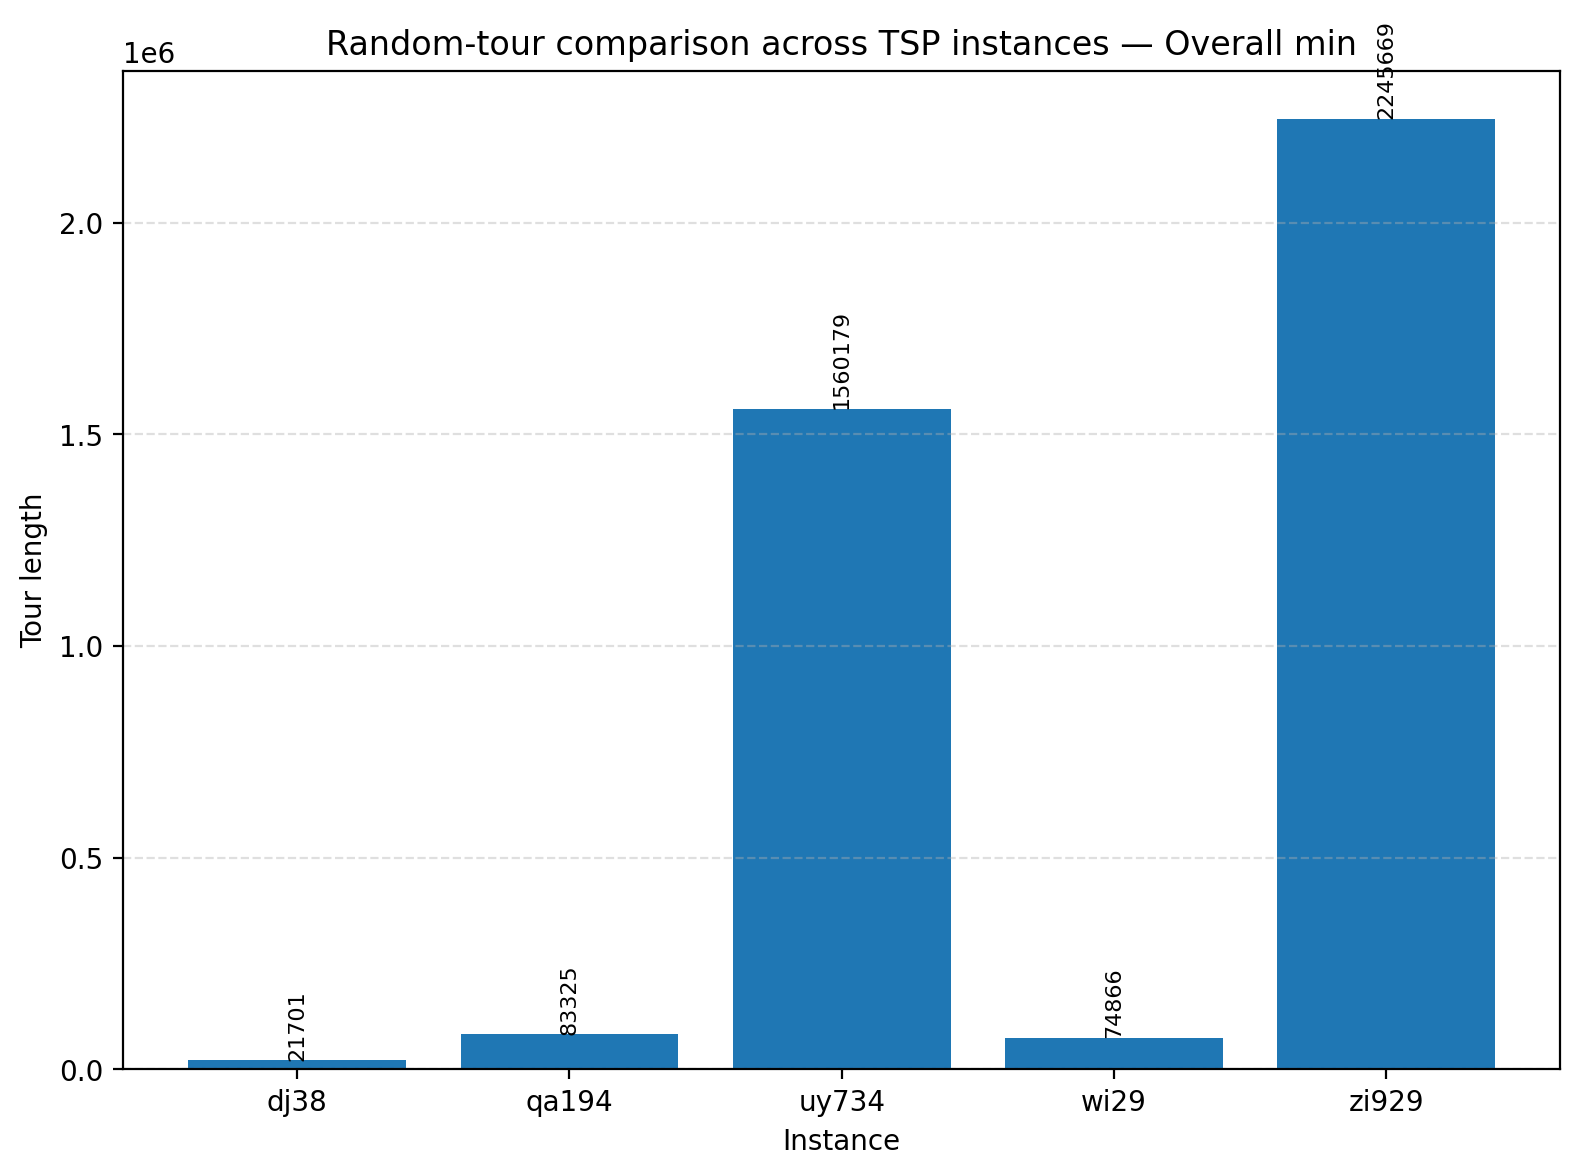
\includegraphics[width=0.86\textwidth]{plots_stats/overall_min.png}
    \caption{Porównanie minimum globalnego spośród \num{1000} losowań.}
    \label{fig:overall}
\end{figure}

\section{Wizualizacje MST i cyklu MST+DFS}
Na kolejnych rysunkach po lewej stronie pokazano minimalne drzewo rozpinające (czerwone),
a po prawej cykl zbudowany metodą DFS po MST (niebieski). Dla małych instancji geometria
jest czytelna od razu; dla dużych instancji najważniejsze staje się ogólne dopasowanie trasy do
kształtu chmury punktów.

\begin{figure}[H]
    \centering
    \begin{subfigure}[t]{0.48\textwidth}
        \centering
        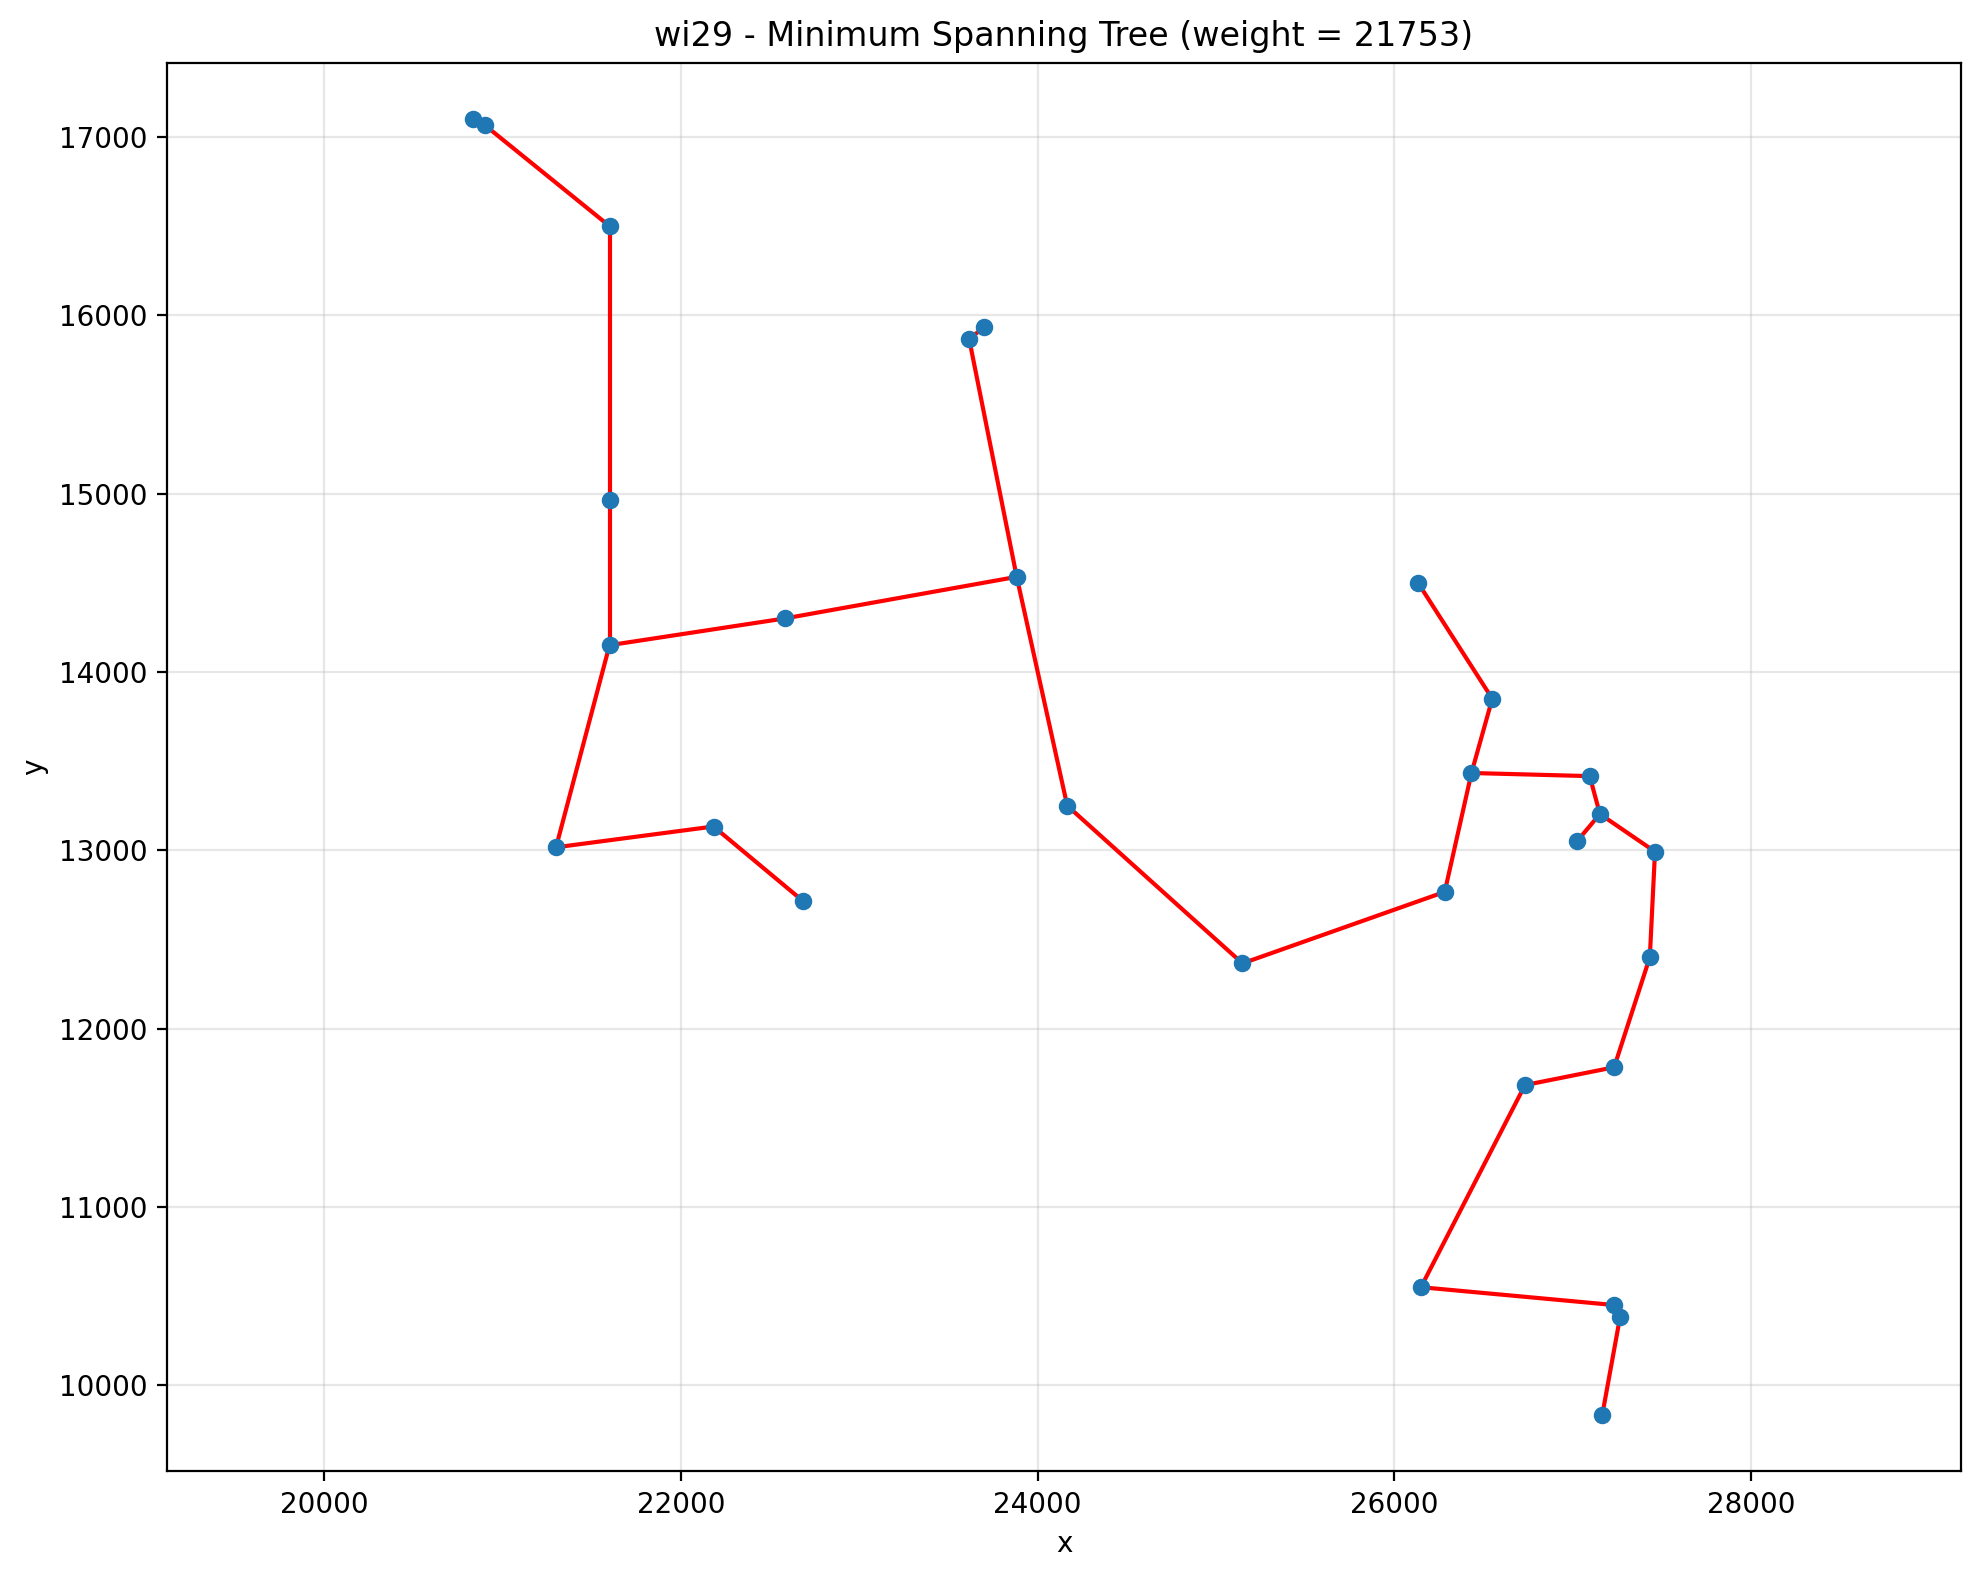
\includegraphics[width=\textwidth]{plots/wi29_mst.png}
        \caption{MST dla \texttt{wi29}}
    \end{subfigure}
    \hfill
    \begin{subfigure}[t]{0.48\textwidth}
        \centering
        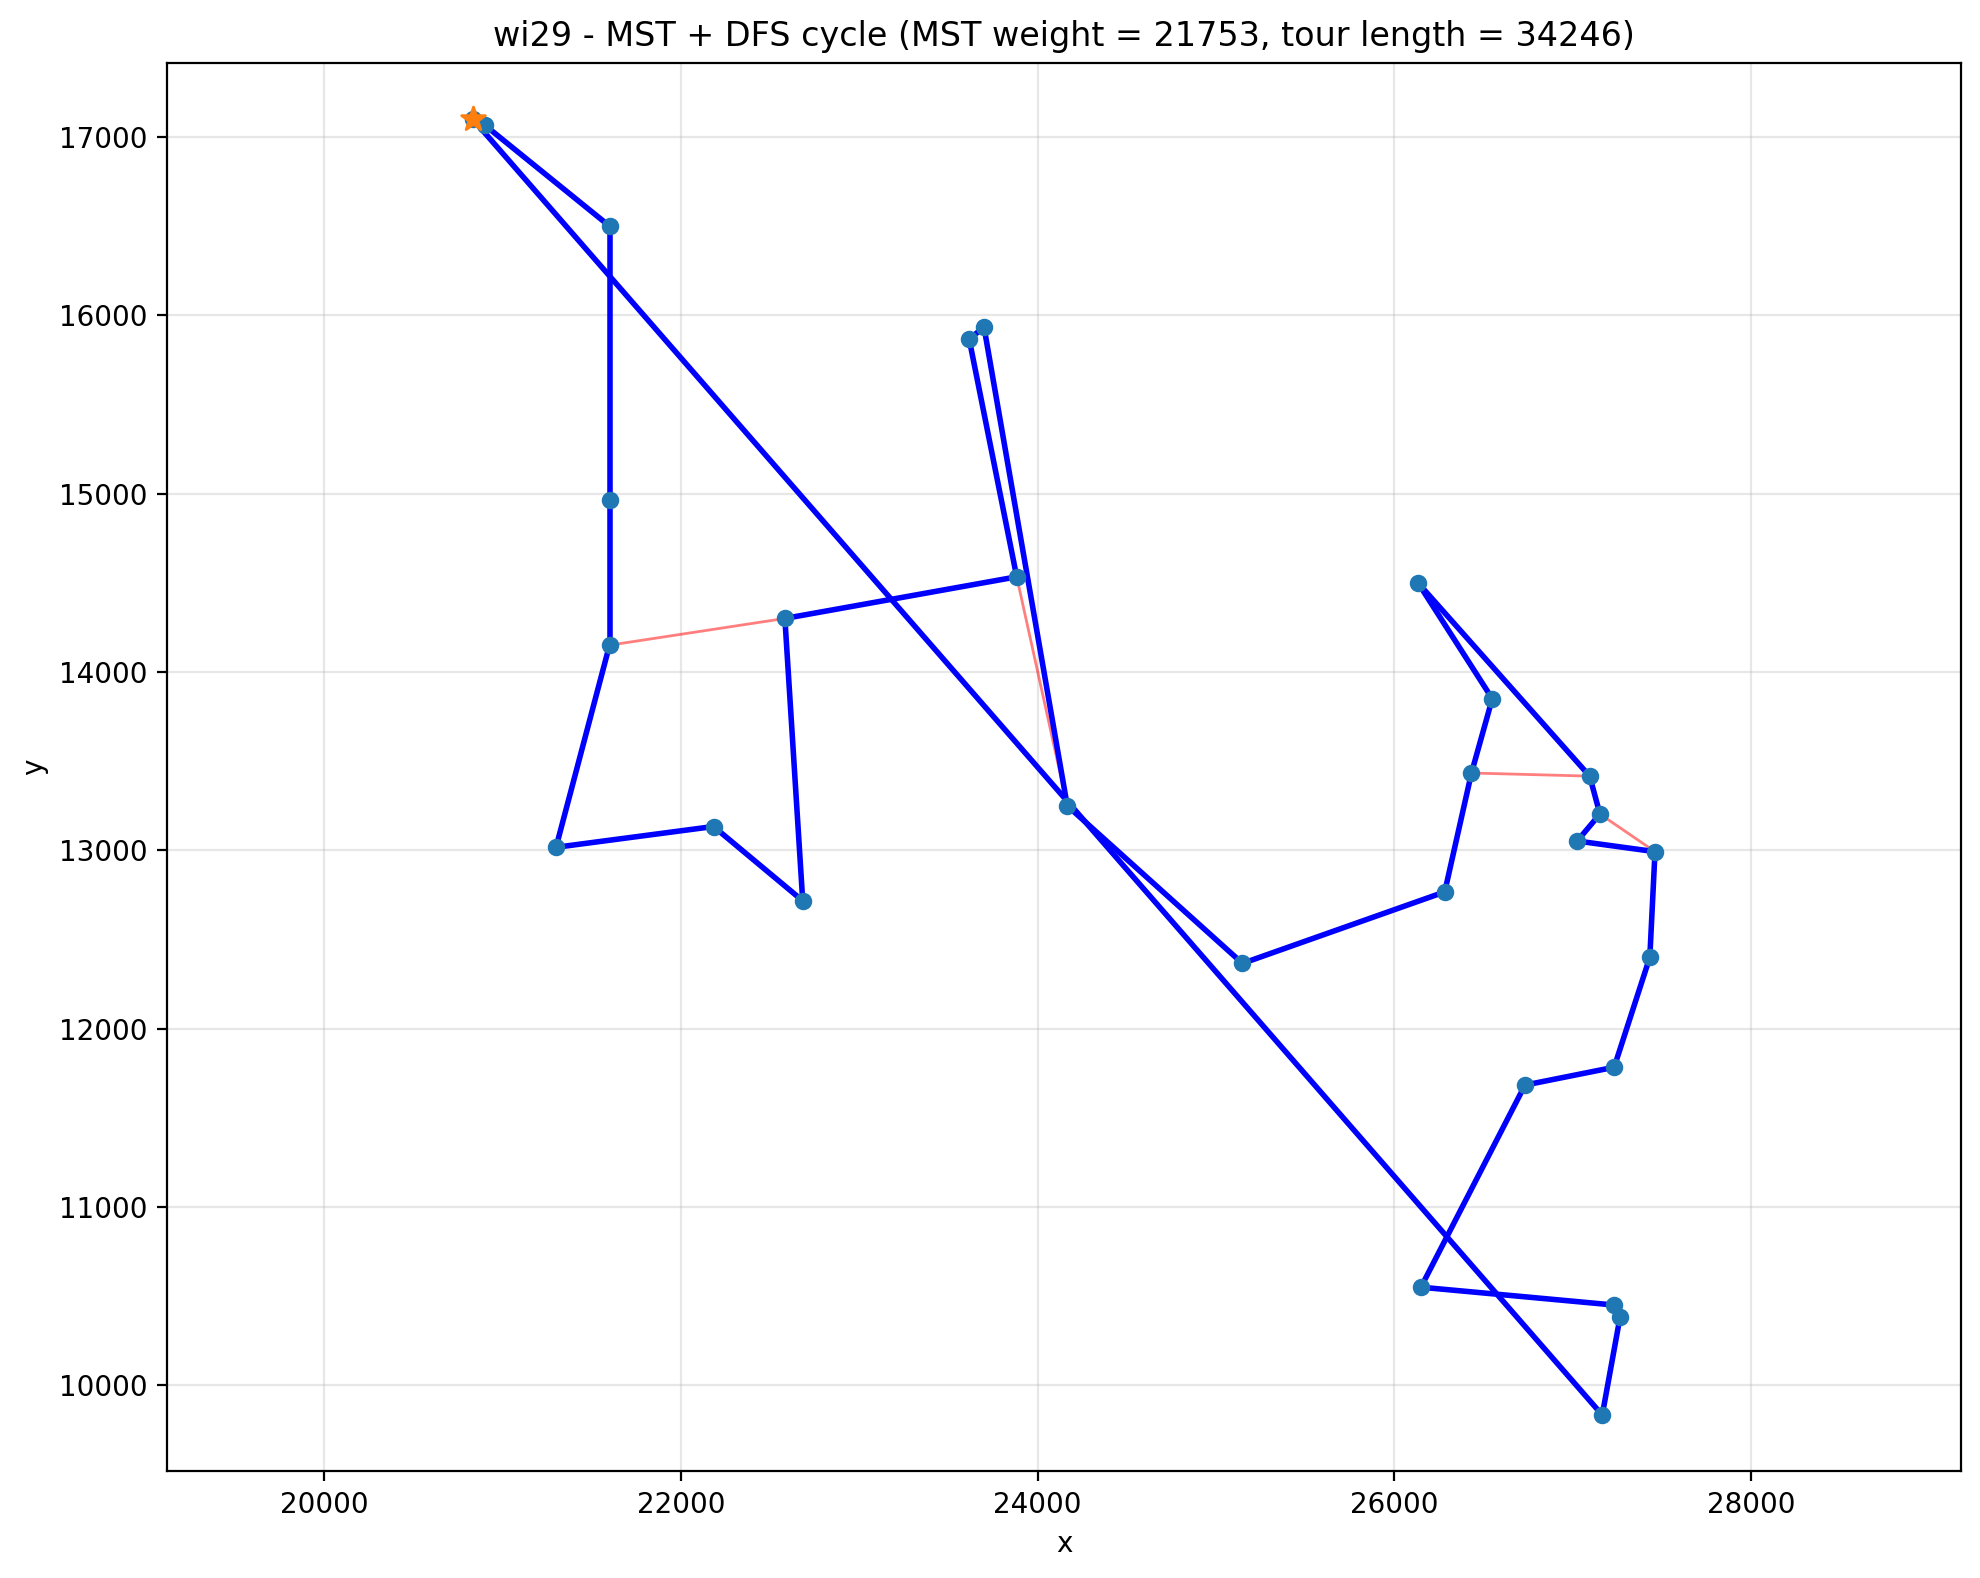
\includegraphics[width=\textwidth]{plots/wi29_mst_dfs_cycle.png}
        \caption{Cykl MST+DFS dla \texttt{wi29}}
    \end{subfigure}
    \caption{Western Sahara.}
\end{figure}

\begin{figure}[H]
    \centering
    \begin{subfigure}[t]{0.48\textwidth}
        \centering
        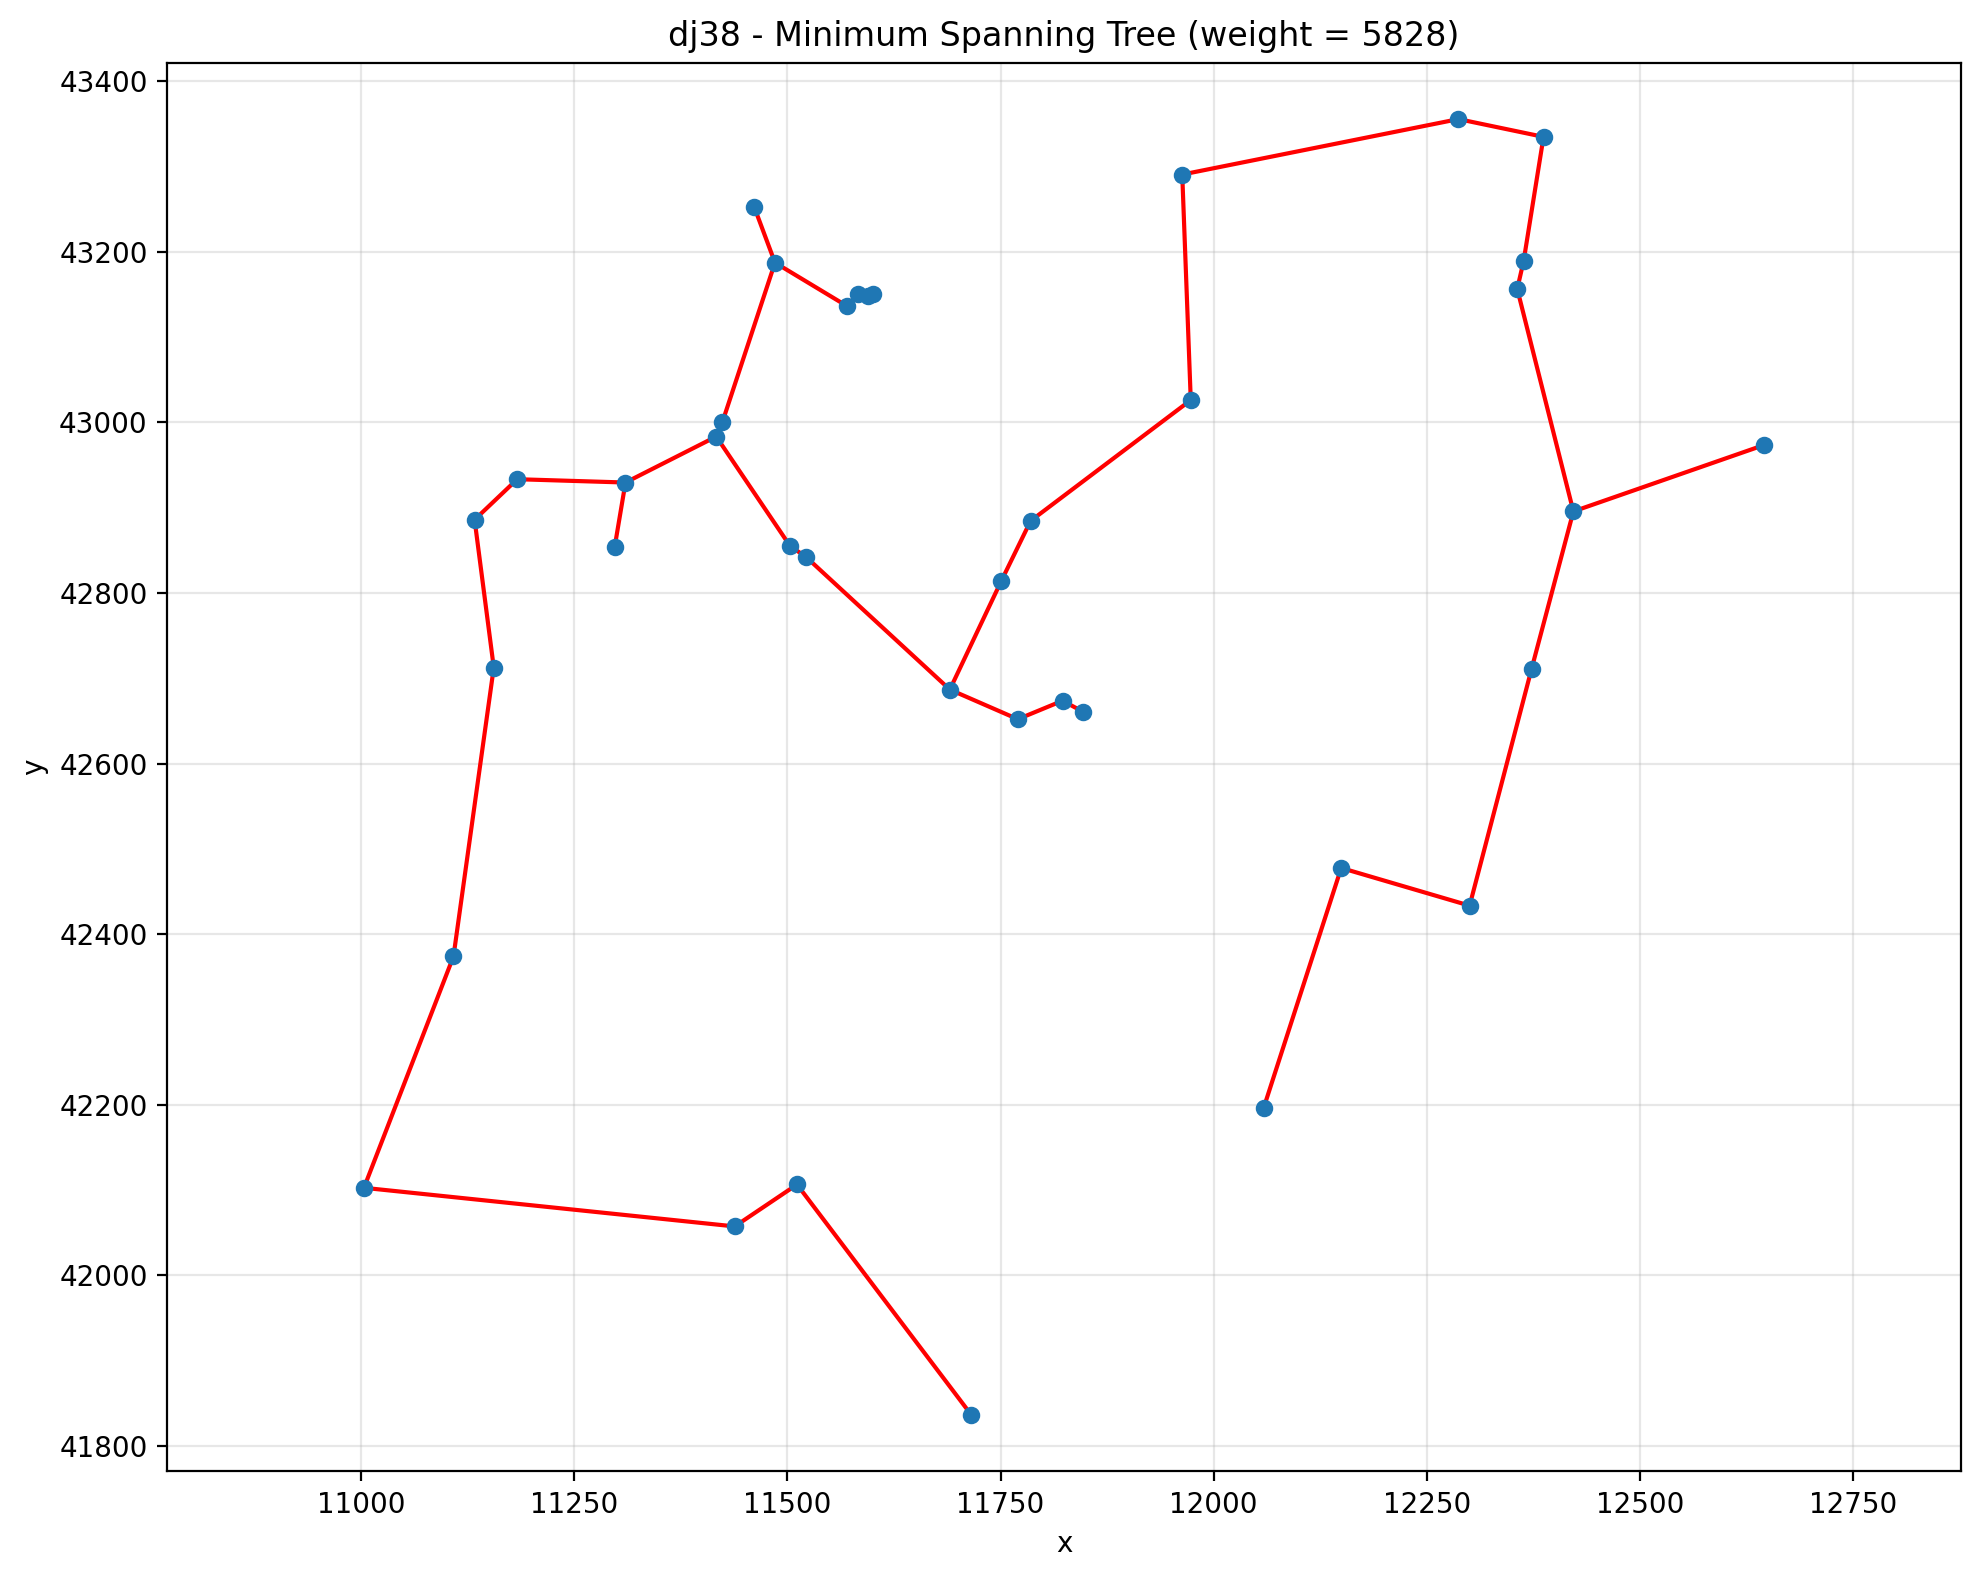
\includegraphics[width=\textwidth]{plots/dj38_mst.png}
        \caption{MST dla \texttt{dj38}}
    \end{subfigure}
    \hfill
    \begin{subfigure}[t]{0.48\textwidth}
        \centering
        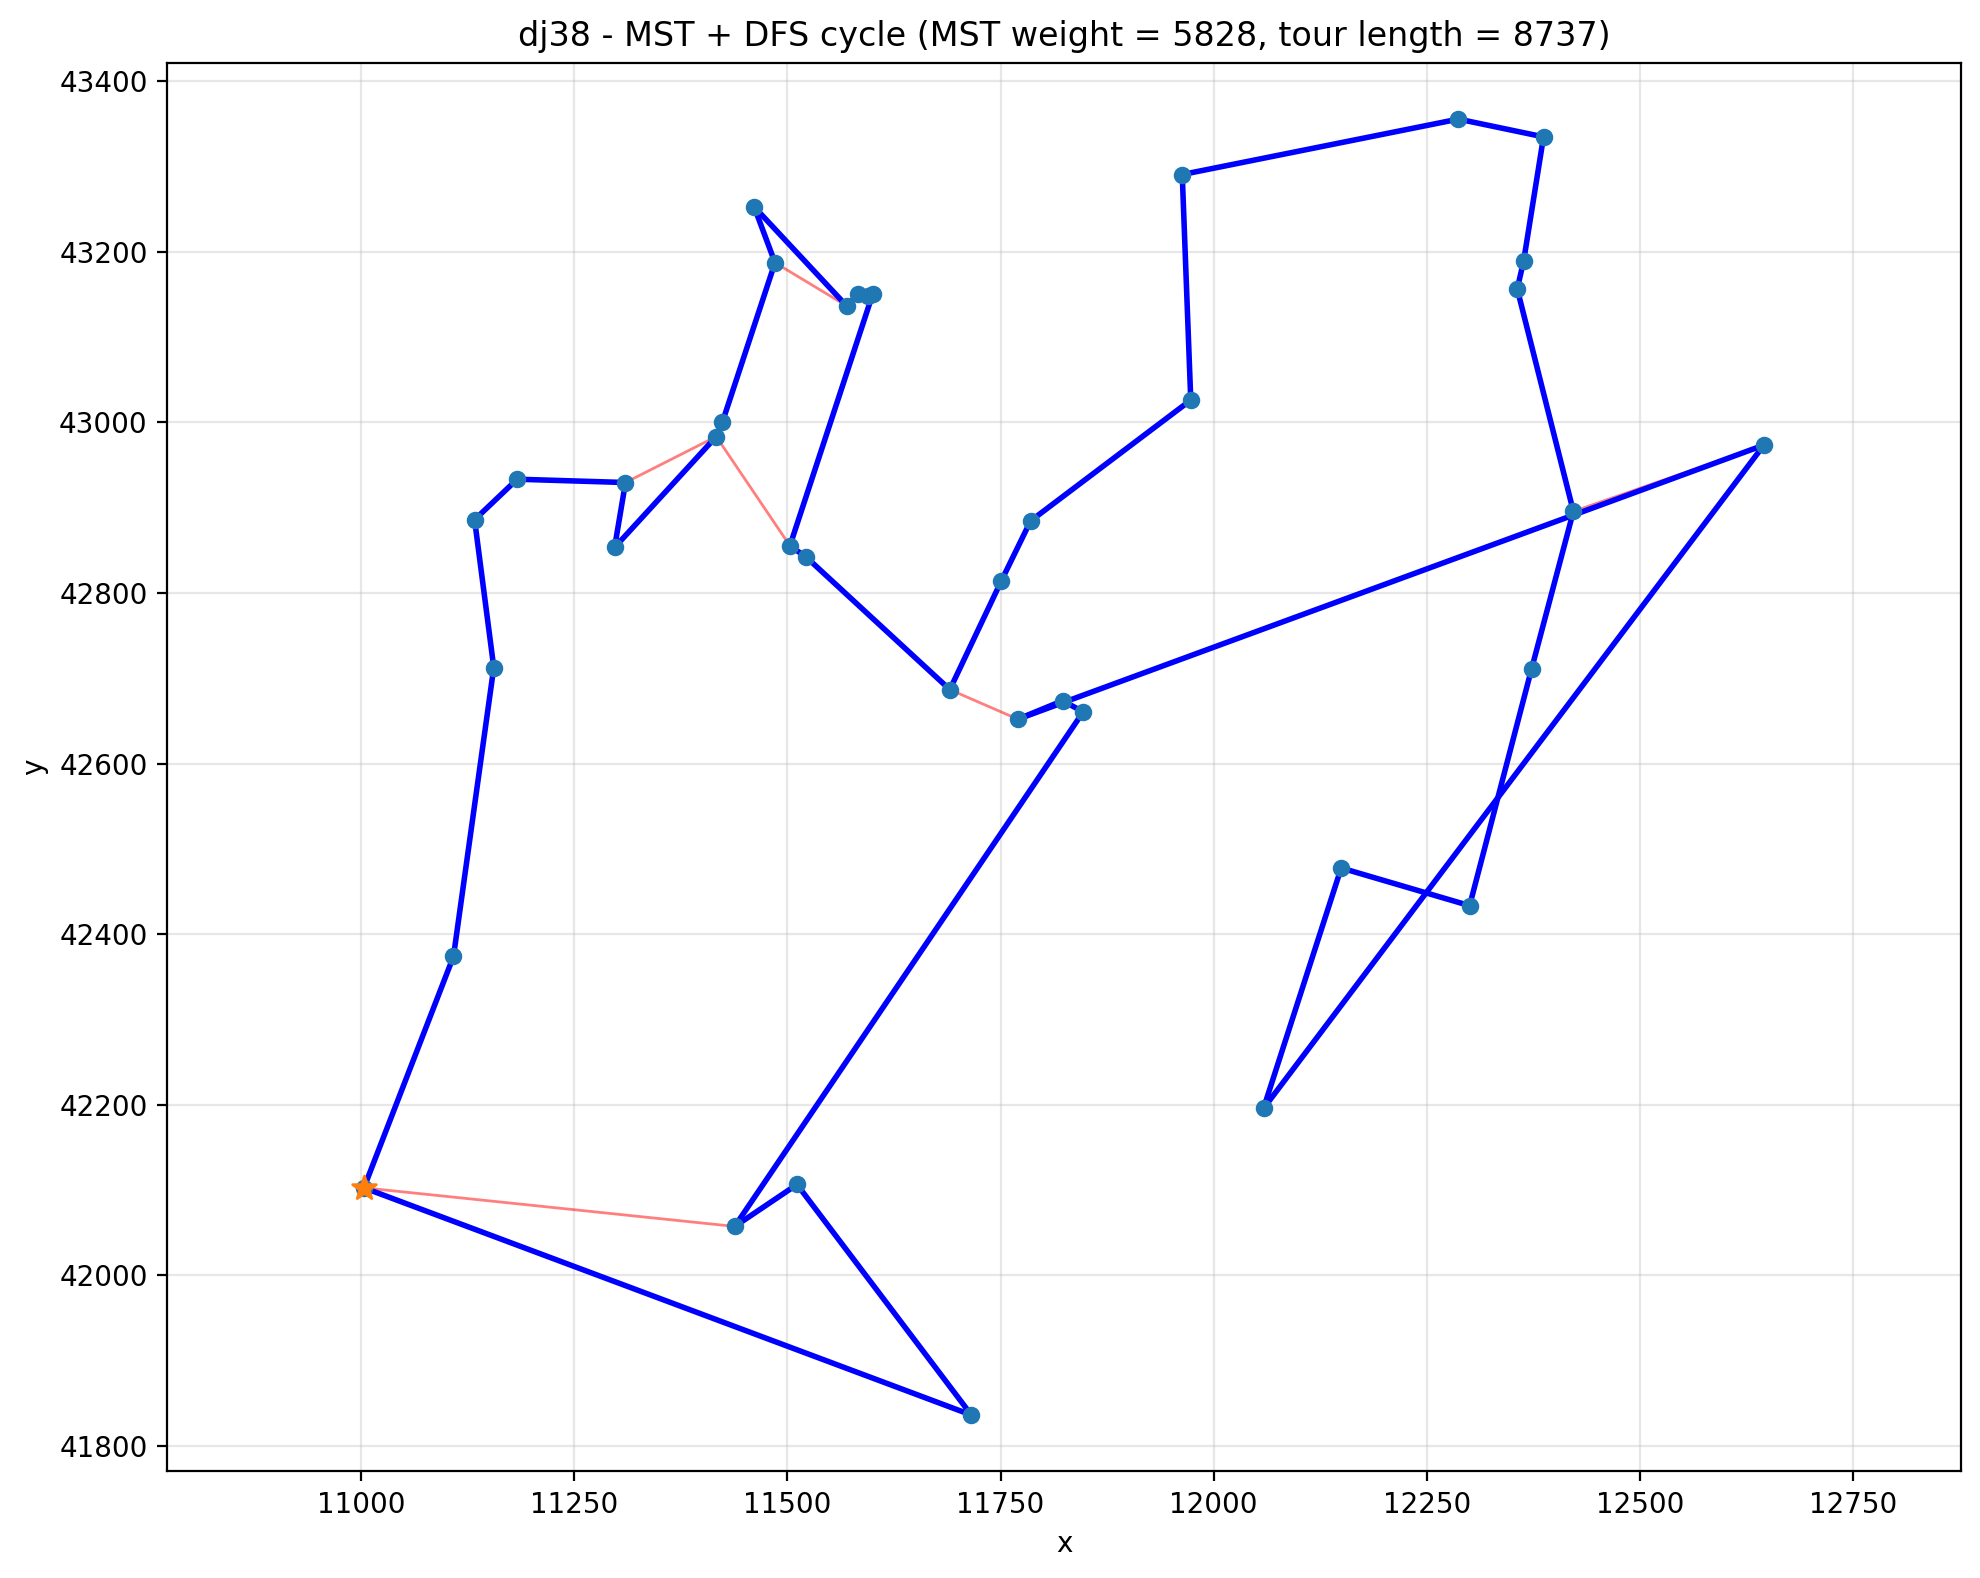
\includegraphics[width=\textwidth]{plots/dj38_mst_dfs_cycle.png}
        \caption{Cykl MST+DFS dla \texttt{dj38}}
    \end{subfigure}
    \caption{Dżibuti.}
\end{figure}

\begin{figure}[H]
    \centering
    \begin{subfigure}[t]{0.48\textwidth}
        \centering
        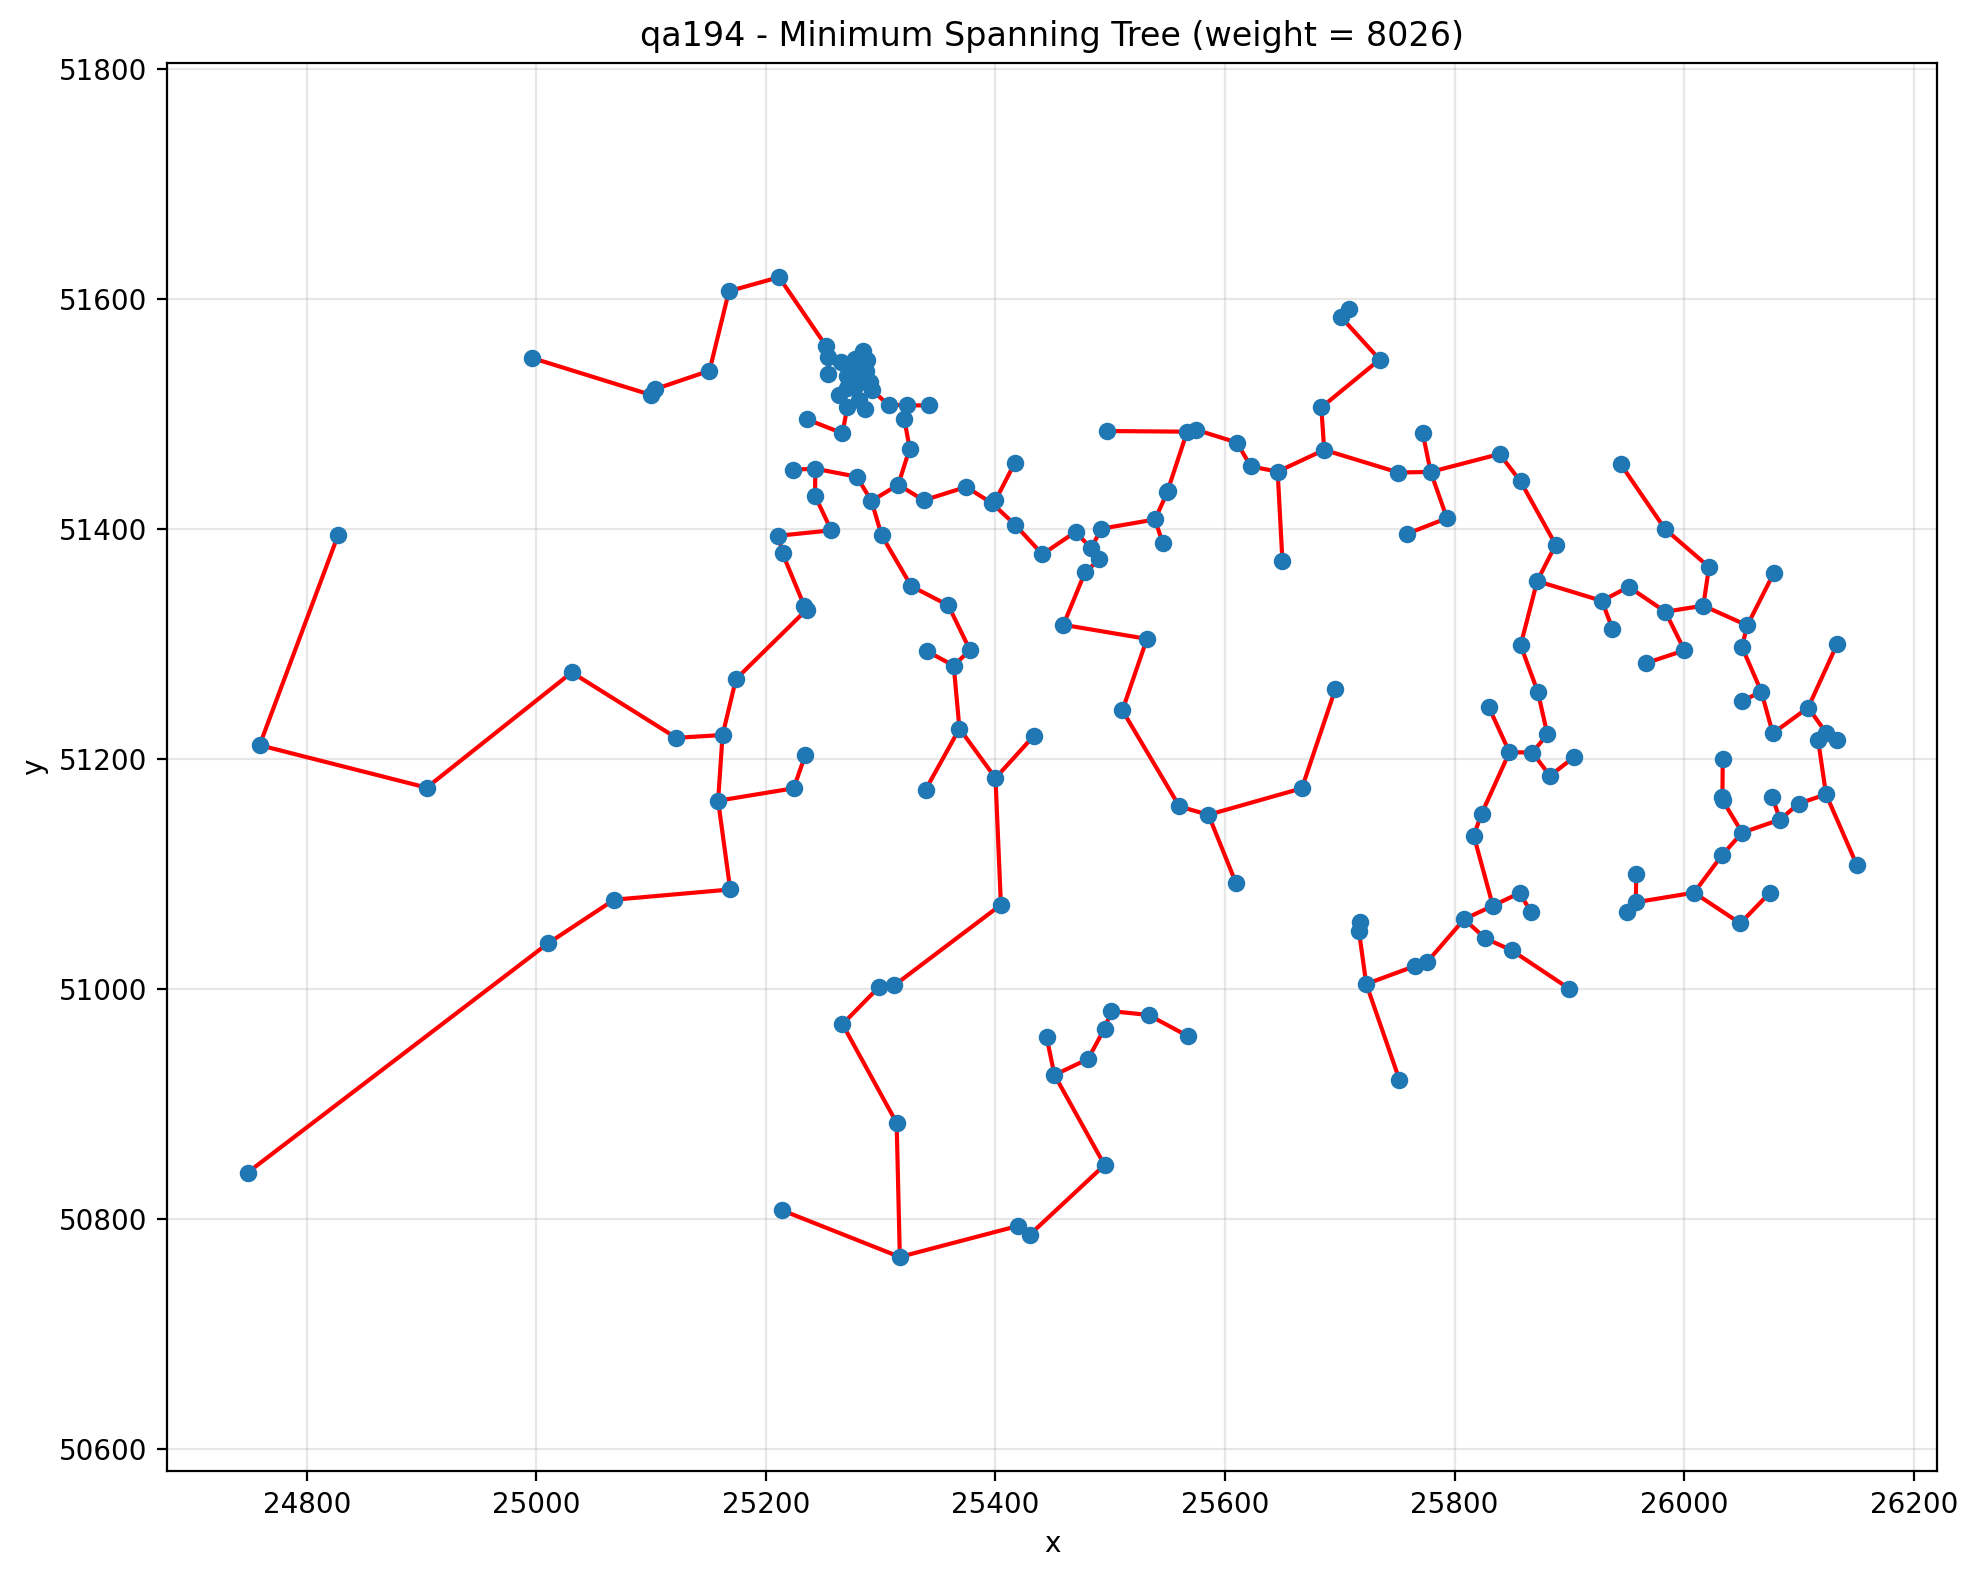
\includegraphics[width=\textwidth]{plots/qa194_mst.png}
        \caption{MST dla \texttt{qa194}}
    \end{subfigure}
    \hfill
    \begin{subfigure}[t]{0.48\textwidth}
        \centering
        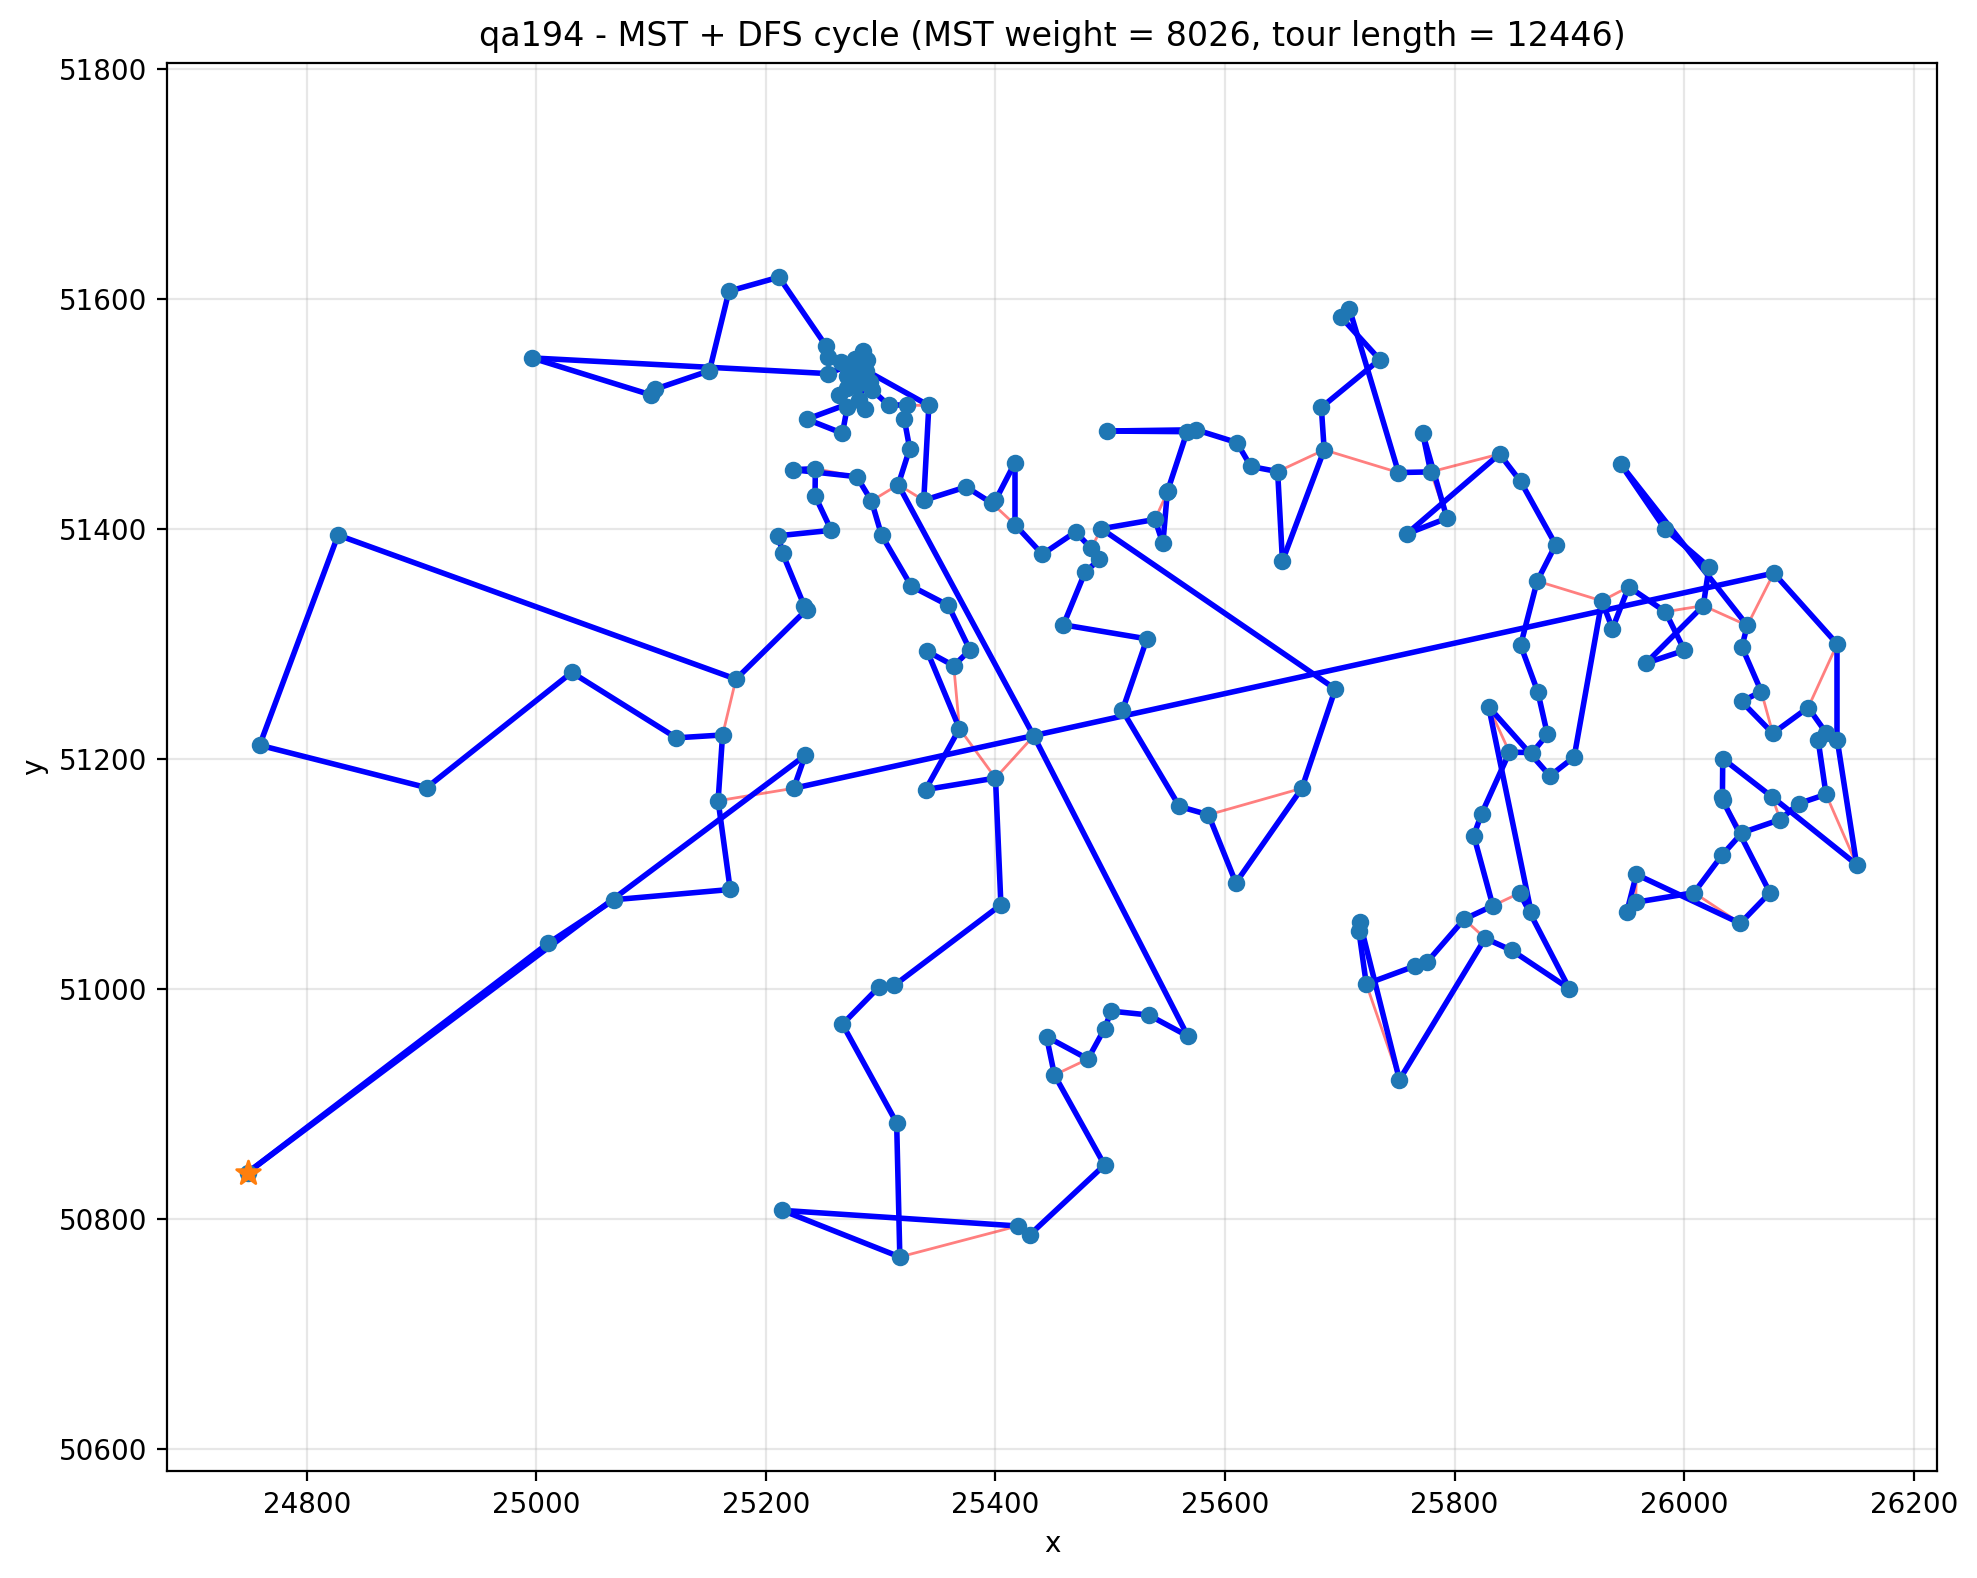
\includegraphics[width=\textwidth]{plots/qa194_mst_dfs_cycle.png}
        \caption{Cykl MST+DFS dla \texttt{qa194}}
    \end{subfigure}
    \caption{Katar.}
\end{figure}

\begin{figure}[H]
    \centering
    \begin{subfigure}[t]{0.48\textwidth}
        \centering
        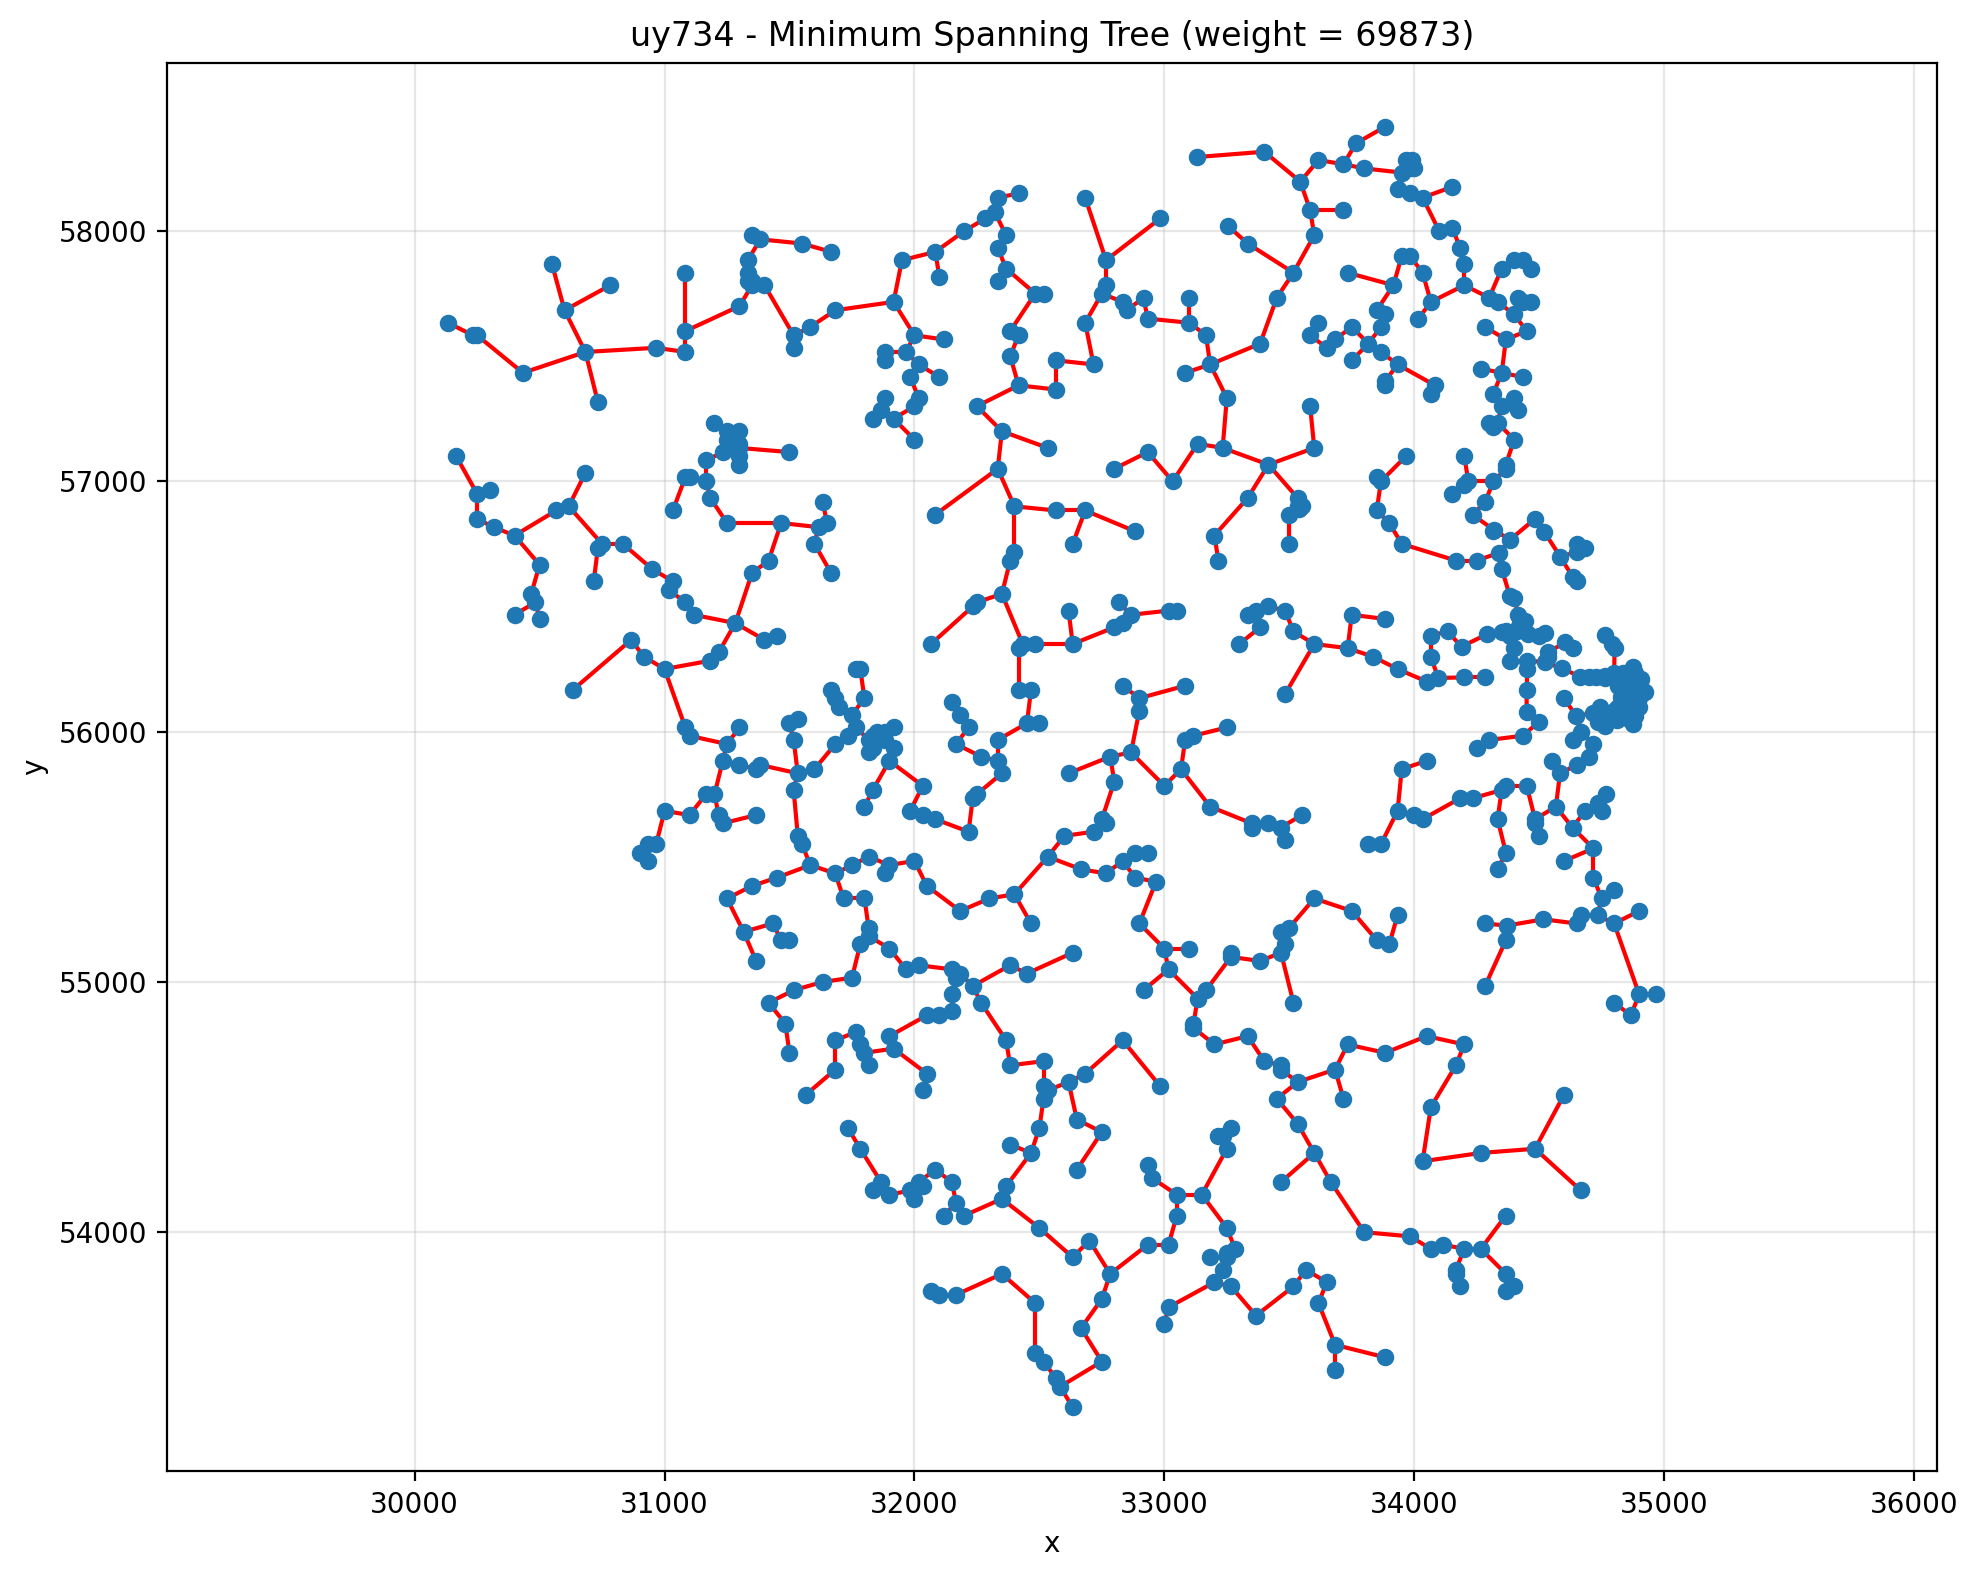
\includegraphics[width=\textwidth]{plots/uy734_mst.png}
        \caption{MST dla \texttt{uy734}}
    \end{subfigure}
    \hfill
    \begin{subfigure}[t]{0.48\textwidth}
        \centering
        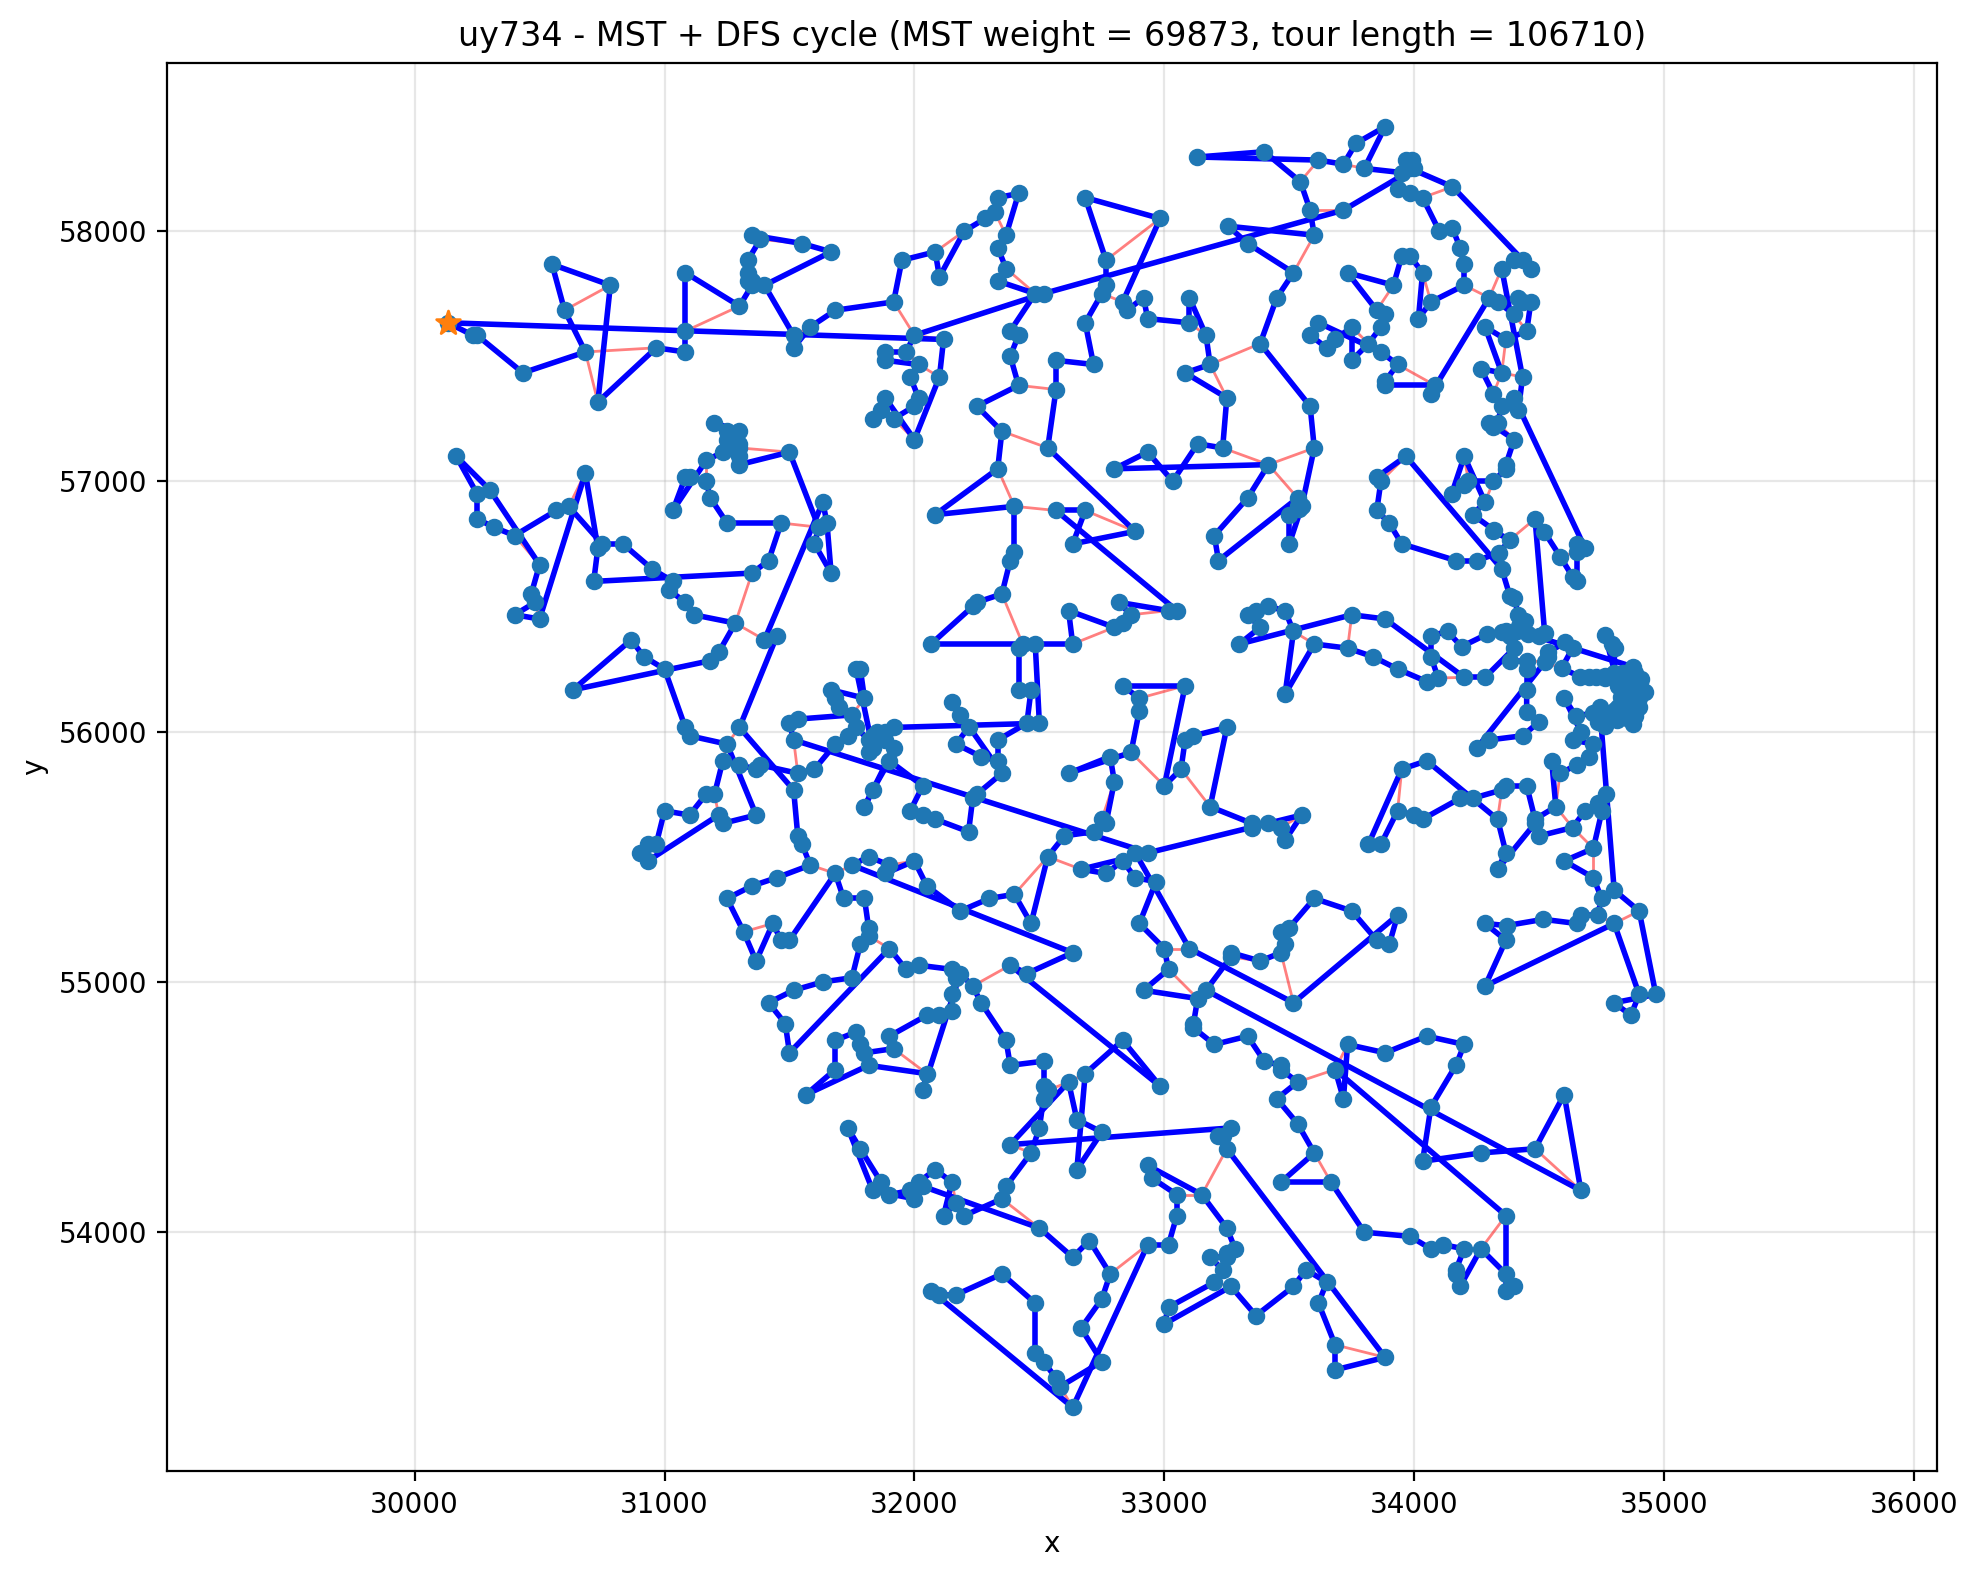
\includegraphics[width=\textwidth]{plots/uy734_mst_dfs_cycle.png}
        \caption{Cykl MST+DFS dla \texttt{uy734}}
    \end{subfigure}
    \caption{Urugwaj.}
\end{figure}

\begin{figure}[H]
    \centering
    \begin{subfigure}[t]{0.48\textwidth}
        \centering
        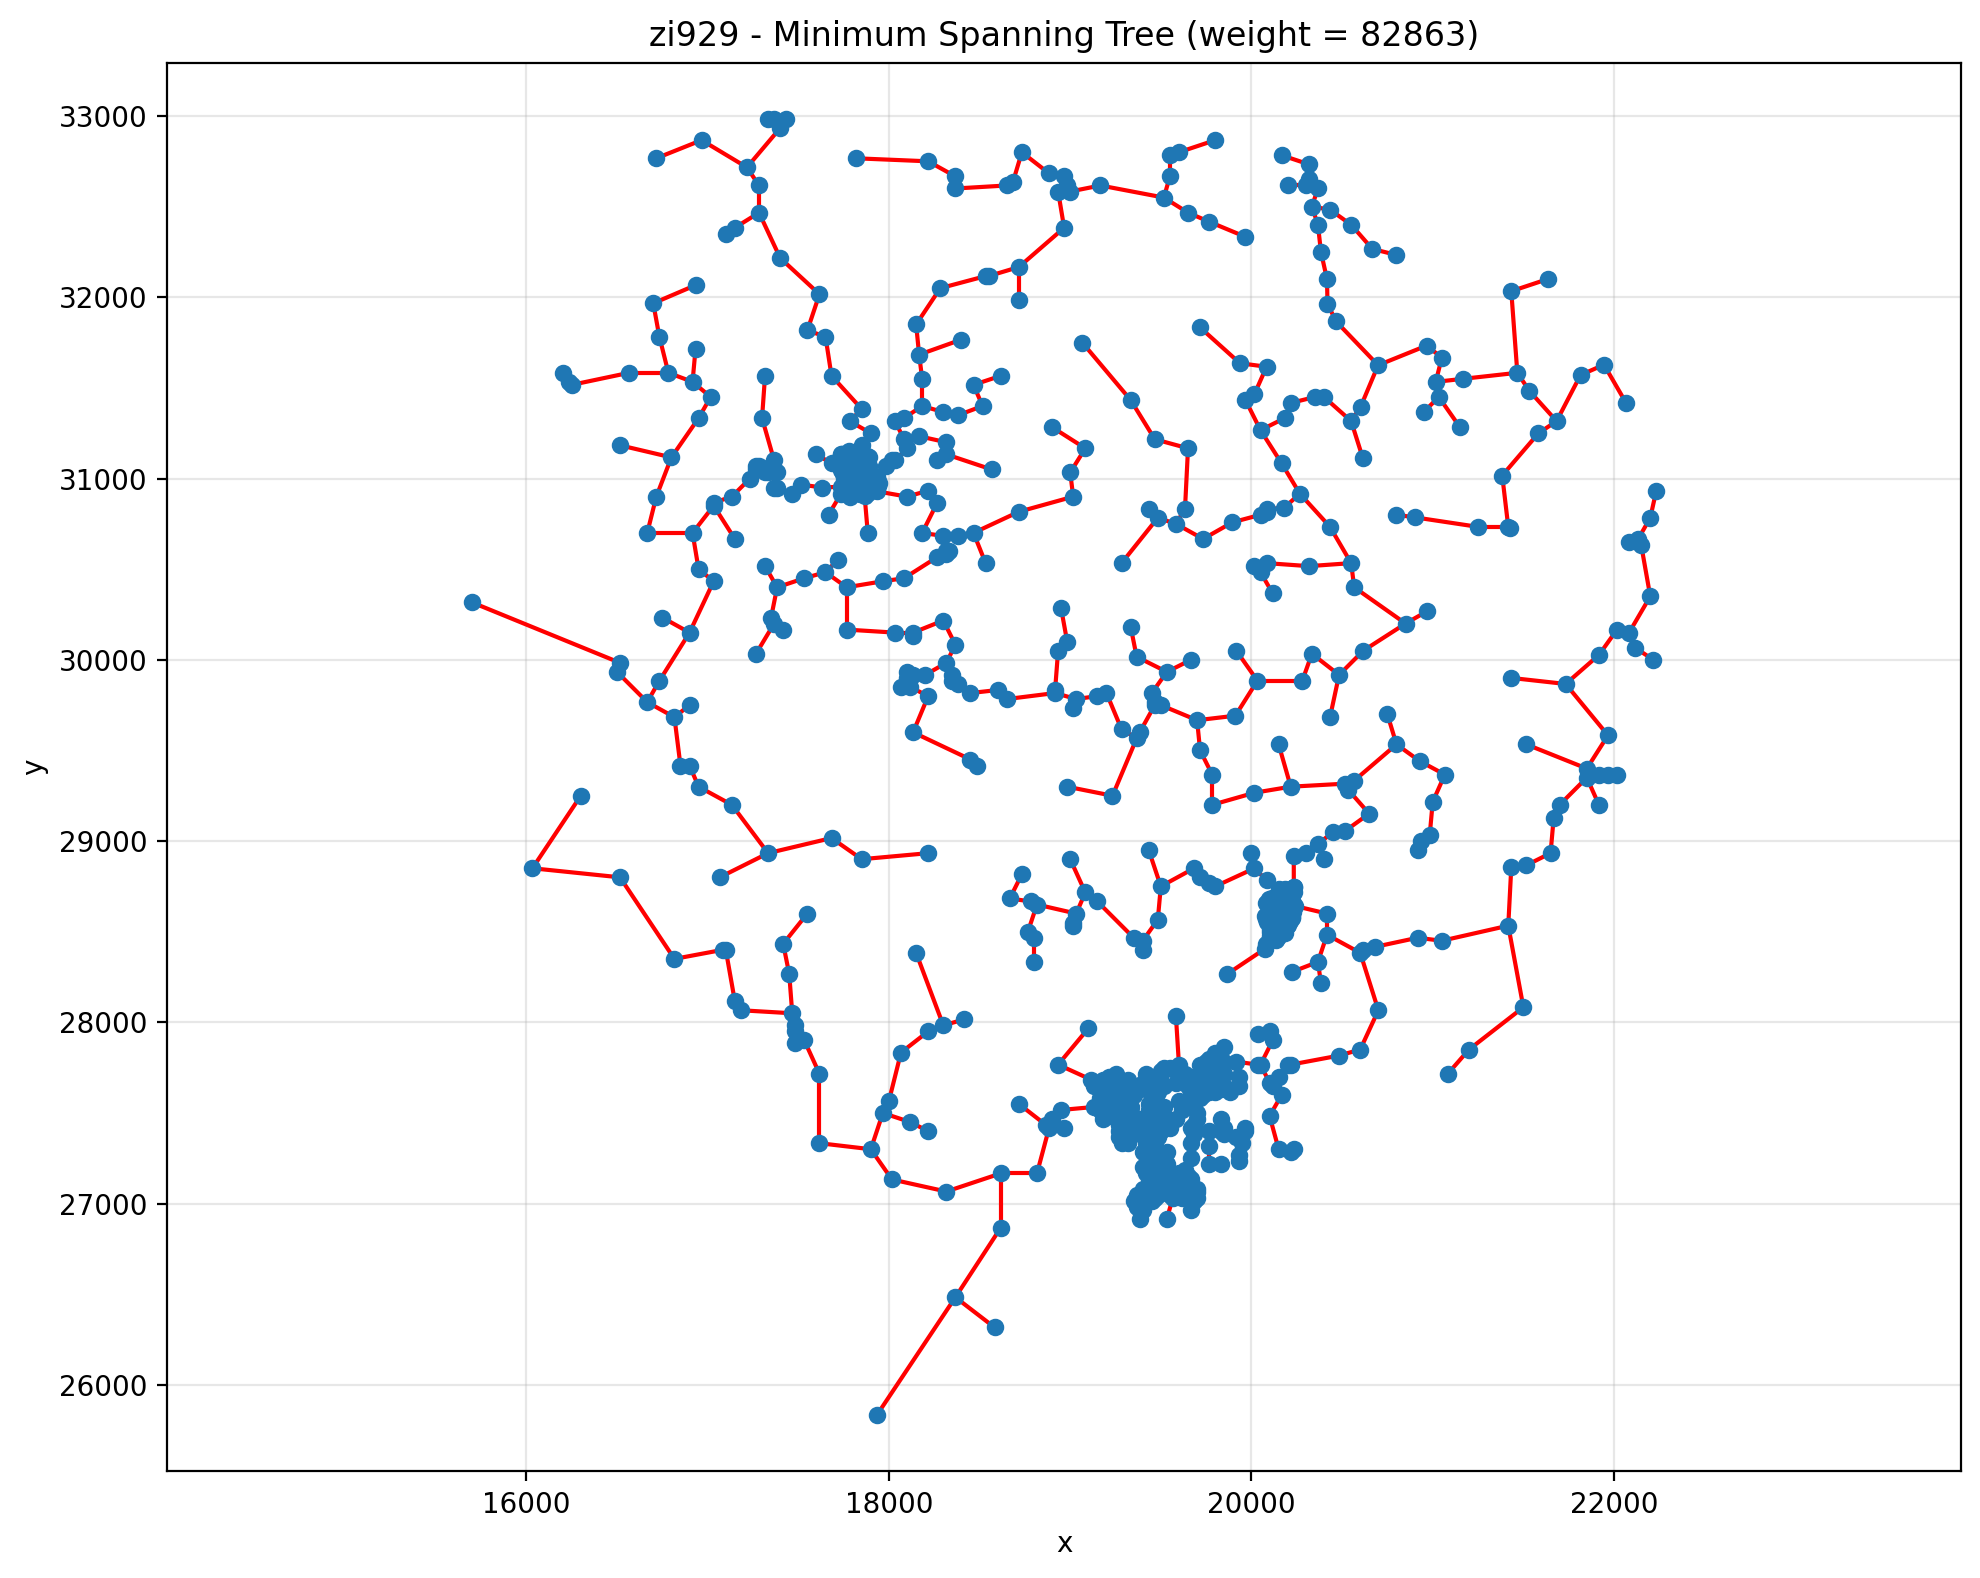
\includegraphics[width=\textwidth]{plots/zi929_mst.png}
        \caption{MST dla \texttt{zi929}}
    \end{subfigure}
    \hfill
    \begin{subfigure}[t]{0.48\textwidth}
        \centering
        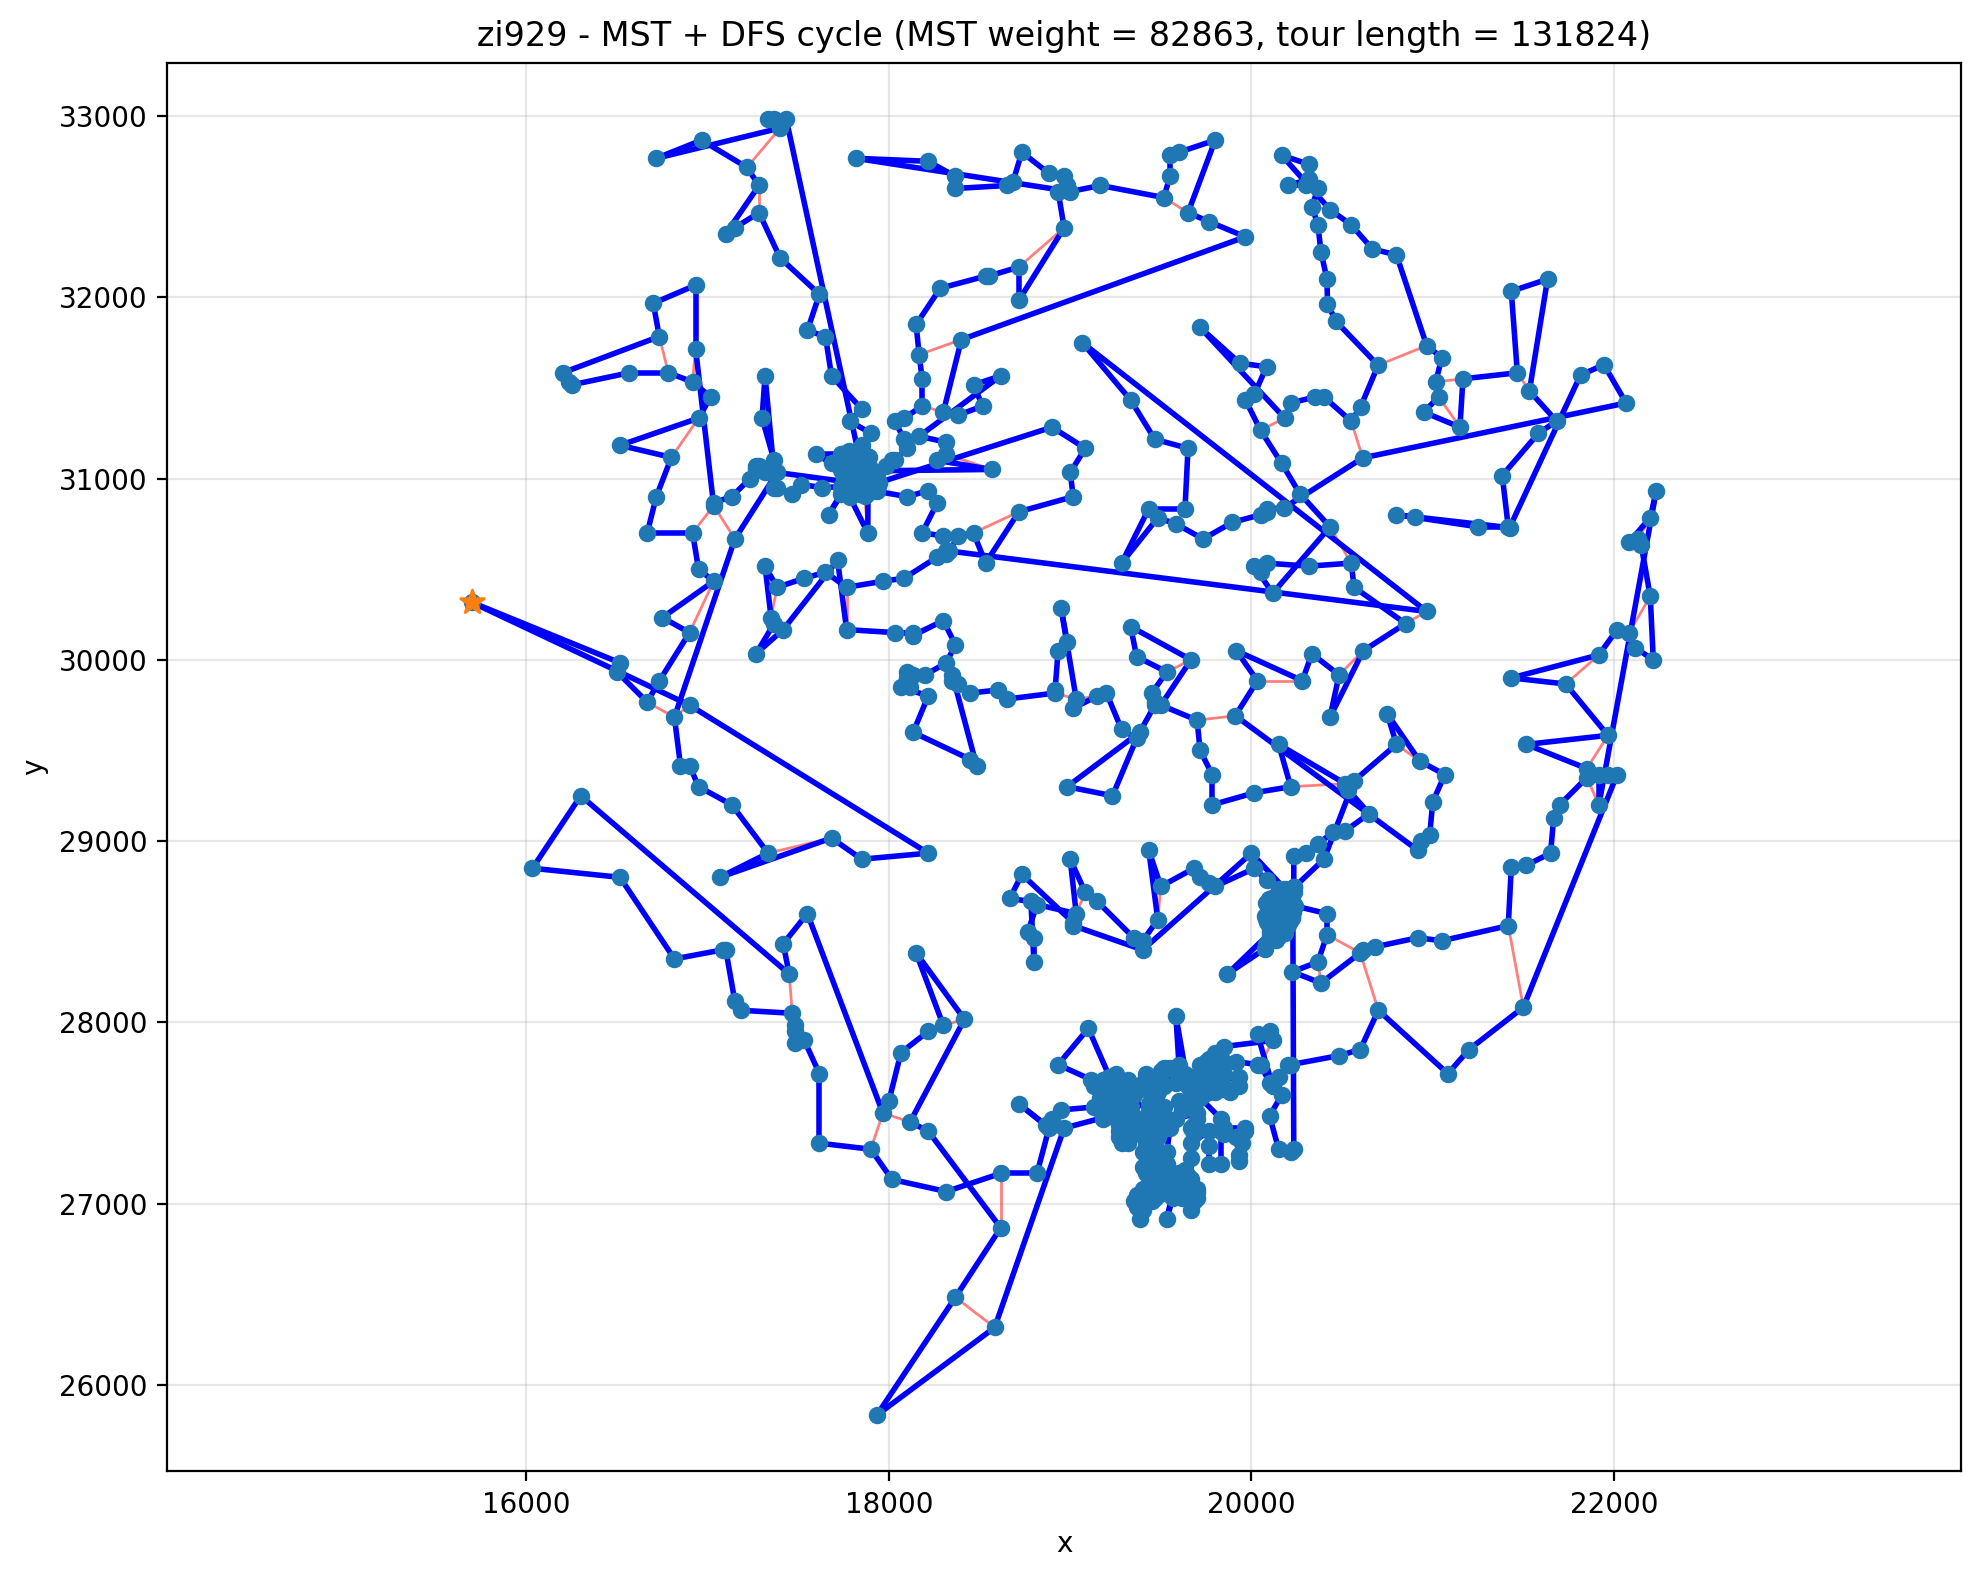
\includegraphics[width=\textwidth]{plots/zi929_mst_dfs_cycle.png}
        \caption{Cykl MST+DFS dla \texttt{zi929}}
    \end{subfigure}
    \caption{Zimbabwe.}
\end{figure}

\section{Omówienie wyników}
Wyniki pokazują, że sama losowość praktycznie nie rozwiązuje problemu TSP.
Dla małych instancji, takich jak \texttt{dj38} i \texttt{wi29}, najlepszy cykl spośród \num{1000}
losowań nadal jest ponad dwukrotnie gorszy od optimum. Dla większych instancji różnica robi się
drastyczna: dla \texttt{qa194} minimum globalne jest niemal \num{8.83} razy większe od optimum,
dla \texttt{uy734} około \num{19.73} razy, a dla \texttt{zi929} aż około \num{23.36} razy.

Jednocześnie heurystyka MST+DFS daje wyniki znacznie sensowniejsze.
Koszt otrzymanego cyklu jest dla wszystkich pięciu instancji mniejszy od \(2\,w(\mathrm{MST})\),
co było oczekiwane z teorii. Co więcej, względna luka do optimum pozostaje umiarkowana:
od około \num{24.07}\,\% dla \texttt{wi29} do około \num{38.26}\,\% dla \texttt{zi929}.
To nadal wynik daleki od optimum, ale nieporównanie lepszy niż podejście losowe.

Patrząc na rysunki widać też, skąd bierze się dalsza przestrzeń do poprawy.
Cykl MST+DFS zachowuje ogólną strukturę geometryczną danych, ale zawiera wiele długich połączeń
wynikających z kolejności odwiedzin w DFS. W przestrzeni euklidesowej aż prosi się o późniejszą
lokalną poprawę metodą 2-opt lub 3-opt, czyli przez usuwanie przecięć oraz skracanie zbyt długich
przeskoków między fragmentami trasy. To jest najprostszy kierunek ulepszenia względem rozwiązania
wyjściowego z laboratorium.

\section{Wnioski}
\begin{enumerate}
    \item Losowanie \num{1000} permutacji daje bardzo słabe wyniki i nie skaluje się wraz z rozmiarem instancji.
    \item Statystyka ``20 grup po 50'' jest konsekwentnie lepsza od ``100 grup po 10'', ponieważ minimum wybierane jest z większej liczby prób.
    \item MST stanowi dobre dolne przybliżenie struktury rozwiązania; jego waga jest wyraźnie mniejsza od optimum, co zgadza się z teorią.
    \item Cykl zbudowany przez DFS po MST jest sensowną 2-aproksymacją: w każdej instancji koszt był mniejszy od \(2\,w(\mathrm{MST})\).
    \item W wariancie euklidesowym można łatwo poprawiać trasy przez usuwanie przecięć krawędzi i lokalne operacje typu 2-opt.
\end{enumerate}


\end{document}
